% -----------------------------------------
% ---- Configuración
% -----------------------------------------
\documentclass[runningheads, twocolumn]{llncs}
\usepackage[top=2.2cm, bottom=2.0cm, left=2.5cm, right=2.5cm]{geometry}
\usepackage{hyperref}
% \usepackage[spanish]{babel}
\usepackage[utf8]{inputenc}
\usepackage{graphicx}
\usepackage{amsmath}
\usepackage[]{subcaption}
\usepackage{listings}
\usepackage{xcolor}
\usepackage[ruled,vlined]{algorithm2e}
\usepackage[font=scriptsize]{caption}
\usepackage{booktabs} % To thicken table lines
\captionsetup[table]{position=bottom, skip=10pt}
% \spanishdecimal{.} % Cambia la , decimal por el .
\newcommand{\floor}[1]{\lfloor #1 \rfloor}
\usepackage{emoji}

\begin{document}


\title{\textbf{VizWiz-VQA disaggregation: A new set\\ of visual question classes.}}
\author{
\emoji{man-scientist-light-skin-tone} \textbf{Hernán J. Maina}\inst{1,2} \and \emoji{woman-detective-light-skin-tone} \textbf{Laura Alonso Alemany}\inst{1,2} }

\institute{
    Universidad Nacional de Córdoba \and CONICET, Argentina \\
    \email{hernan.maina@mi.unc.edu.ar}, \email{alemany@unc.edu.ar}
}

\authorrunning{VizWiz-VQA disaggregation.}
\maketitle
\begin{abstract}
% \emph{VizWiz-VQA\footnote{\url{https://vizwiz.org/tasks-and-datasets/vqa/}} (of english, VizWiz Visual Question Answering), es el primer conjunto de datos de respuestas a preguntas visuales confeccionado íntegramente por y para personas con impedimentos visuales. El mismo, estructura sus preguntas en cuatro categorías, donde `other' es la clase predominante con alrededor del 65\%, seguida de un notable conjunto de preguntas ($\sim$27\%) catalogadas como `no respondibles'. En este trabajo, mediante la exploración de diferentes estrategias de clusterización y análisis morfo-sintácticos, se presenta y propone un nuevo conjunto de ocho categorías principales, las cuales son utilizadas para fine-tunear un modelo de clasificación y poder analizar el conjunto de datos original desde una nueva perspectiva. Cabe destacar que esta investigación hace a un lado la modalidad visual `V', para centrarse en la parte `QA' de VQA, con el objetivo de desagregar las clases mayoritarias, para facilitar la comprensión de la naturaleza de las preguntas, y las causas que llevan a que gran parte de ellas no puedan ser respondidas.}
% \end{abstract}

\emph{VizWiz-VQA (VizWiz Visual Question Answering), is the first data-set of visual questions answers made for and by blind people. It, structures his questions into four main categories, where `other' is the predominant class with around 65\%, followed by a salient set of questions ($\sim$27\%) classified as `unanswerable'. In this work, through the exploration of different clustering strategies and morpho-syntactic analysis, a new set of eight main categories is presented and proposed, which are used to fine-tune a automatic classification model and in this way to be able to reanalyze the original set from a new perspective. It should be noted that this research sets aside the visual modality 'V', to focus on the 'QA' part of VQA, with the aim of disaggregate the majority classes, to facilitate the understanding of the nature of the questions, and the reasons why many of these questions cannot be answered.}
\end{abstract}

% -----------------------------------------
% ---- Sections
% -----------------------------------------
\section{Introduction}
% VizWiz, es el proyecto responsable de introducir los primeros conjuntos de datos y retos, destinados a motivar la creación de nuevas y mejores tecnología/algoritmos asistenciales de inteligencia artificial, para ayudar a personas con discapacidades visuales.
% En 2010, Bigham et al. [6] presenta VizWiz, una aplicación de teléfono móvil destinada a ayudar a personas no videntes en sus problemas diarios. Los usuarios tomaban una fotografía y grababan una pregunta sobre lo que querían conocer de esa imagen. Tales preguntas visuales, eran respondidas por un grupo de trabajadores, mayoritariamente reclutados de empresas como Amazon Mechanical Turk.
% Ocho años después, Gurari et al. [3] filtraron y anonimizaron la información de todos los datos recopilados hasta ese momento, y para cada par de imágenes y preguntas, recolectaron un total de 10 respuestas provenientes de fuentes múltiples. Esto, llevo a que en la conferencia de Computer Vision and Patter Recognition 2018 (CVPR 18) se presentara el primer conjunto de datos VQA público `orientado a objetivos' no artificial, construido totalmente de datos originados por  personas no videntes. La Figura (\ref{fig:vizwiz_samples}) ilustra algunos ejemplos de esta dataset.
VizWiz\footnote {\url{https://vizwiz.org}}, is the project responsible for introducing the first datasets and challenges, aimed at motivating the creation of new and better AI assistive technology/algorithms, to help people with visual impairment.
In 2010, Bigham et al. \cite{vizwiz_phone} presents VizWiz, a mobile phone application designed to help blind people with their daily problems. Users took a photo and recorded a question about what they wanted to know about that image. Such visual questions were answered by a group of workers, mostly recruited from companies like Amazon Mechanical Turk.
Eight years later, Gurari et al. \cite{vizwiz_grandchallenge} filtered and anonymized the information from all the data collected up to that point, and for each pair of images/questions, they collected a total of 10 answers using crowd-sources. In the Computer Vision and Pattern Recognition 2018 conference (CVPR 18), they presenting the first non-artificial 'goal-oriented' public VQA data-set, built entirely from data originated by blind people. Figure (\ref{fig:vizwiz_samples}) illustrates some examples of this dataset.

\begin{figure}[ht!]
    \centering
    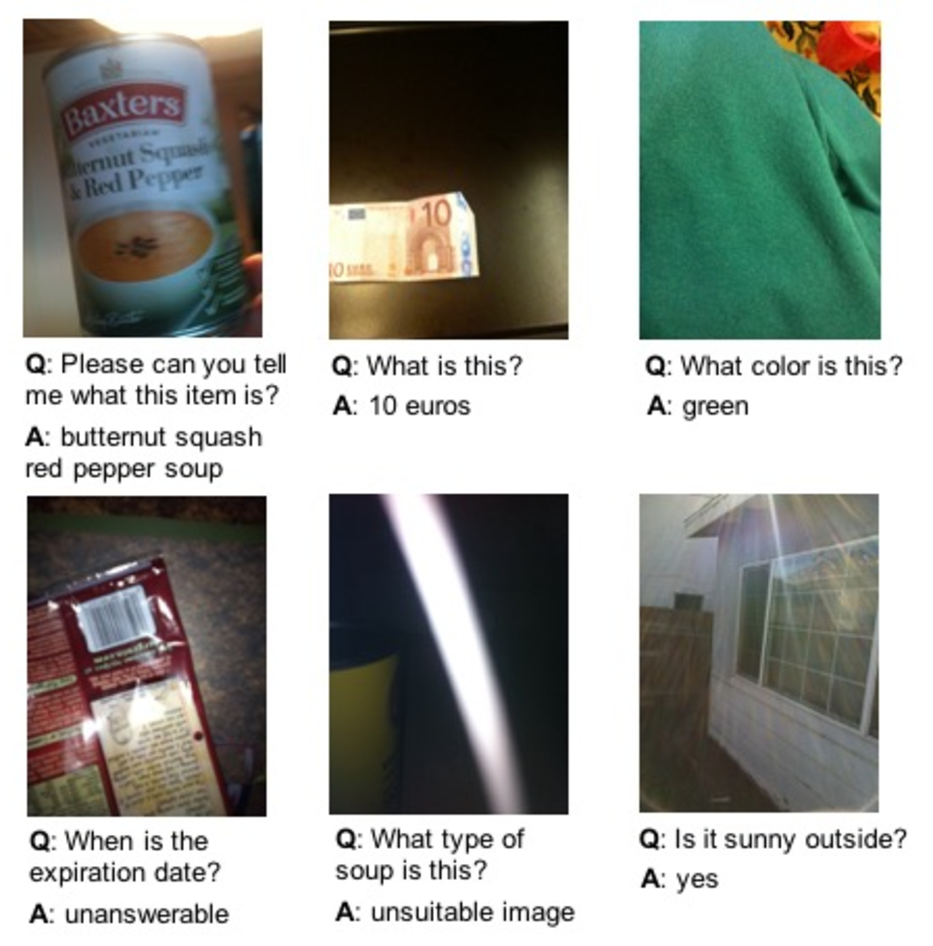
\includegraphics[width=\linewidth]{images/intro/vizwiz_samples.pdf}
\caption{Samples of VizWiz-VQA dataset.}
\label{fig:vizwiz_samples}
\end{figure}


\paragraph{\textbf{VizWiz-VQA.}}
% Dado a que las mismas personas no videntes fueron las responsables de capturar las fotografías y grabar las preguntas, gran parte de las imágenes de este conjunto de datos, se caracterizan por presentar problemas de enfoque, iluminación y encuadre. Por otro lado, las preguntas son marcadamente conversacionales, ya que no se hablan como se escribe, y gran parte de ellas aparecen incompletas como consecuencias de cortes e imperfecciones en los audios de las que fueron transcritas.
% Como resultado, ya sea porque la pregunta no pudo ser respondida del contexto de la imagen, o porque la calidad de la imagen era inadecuada, VizWiz-VQA cuenta con una gran cantidad de preguntas visuales que no pueden ser respondidas, diferenciándolo del resto de datasets VQA.
Since the same blind people were responsible for capturing the photographs and recording the questions, a large part of the images in this data set are characterized by focusing, lighting and framing problems. On the other hand, since people speak differently from how they write, the data set is markedly conversational. With a large majority of incomplete questions due to cuts and imperfections in the audios from which they were transcribed.
As a result, either because the question could not be answered from the context of the image, or because the image quality was unsuitable, VizWiz-VQA has a large number of visual questions that cannot be answered, unlike other VQA datasets.

% Específicamente, el conjunto esta formado por 20523 pares image/question y 205230 respuesta asociadas para el grupo de entrenamiento; 4319 pares de image/question y 43190 respuestas asociadas para el grupo de validación; y 8000 pares de image/question en el grupo de testeo. Cada una de las preguntas poseen asignada una categoría, la cual hereda del tipo de respuesta esperada (los valores entre paréntesis representan la frecuencia en el dataset): `number' ($\sim$1,4\%), `yes/no' ($\sim$4,63\%), `unanswerable' ($\sim$27,84\%) y `other' ($\sim$66,1\%).
% La longitud media de cada pregunta ronda las $\sim$6.8 palabras, y aproximadamente el 28\% de las palabras iniciales aparecen menos del 5\% de la veces en el conjunto. Esto último, atribuido a la naturaleza conversacional del conjunto, donde preguntas del estilo “Hi, can you please tell me which is . . . ” in VizWiz, se encuentra simplemente como “Which is . . . ” en conjunts como VQA v2.0.

Specifically, VizWIz-VQA\footnote {\url{https://vizwiz.org/tasks-and-datasets/vqa/}} is conformed of 20523 images/questions pairs, and 205230 associated answers in the training set; 4319 image/question pairs, and 43190 associated answers in the validation set; and 8000 pairs of images/questions in the test set. Each of the questions is assigned a category, which inherits the type of expected answer (the values in parentheses represent the frequency in the dataset): `number' ($\sim$1,4\%), `yes/no' ($\sim$4.63\%), `unanswerable' ($\sim$27.84\%) and `other' ($\sim$66.1\%).
The average length of each question is around $\sim$6.8 words, and approximately 28\% of the opening words appear less than 5\% of the time in the set. The latter, attributed to the conversational nature of the set, where questions such as ``Hi, can you please tell me which is . . . '' in VizWiz, it is found simply as ``Which is. . . '' in datasets like VQA v2.0\footnote{\url{https://visualqa.org/}}.

\paragraph{\textbf{Contributions.}}
% En este trabajo, como consecuencia del análisis de  $\sim$24800 pares de preguntas y respuestas provenientes de los conjuntos de entrenamiento y validación, se realizaron las siguientes contribuciones:
% \begin{itemize}
%     \item Exploración e identificación de estrategias de pre-procesamiento y clusterización, para la desagregación consistente de grupos de preguntas mayoritarias del conjunto VizWiz-VQA.
%     \item Definición de ocho nuevas categorías, para identificar y caracterizar de una manera más descriptiva y natural, al conjunto total de preguntas de VizWiz-VQA.
%     \item Entrenamiento y testeo de modelo de clasificación automática sobre las nuevas categorías definidas, y análisis de las categorías originaes `other' y `unanswerable' en base a nuevas clasificaciones obtenidas.
% \end{itemize}
In this work, as a consequence of the analysis of $\sim$24.800 pairs of questions and answers from the training and validation sets, the following contributions were made:
\begin{itemize}
    \item Exploration and identification of pre-processing and clustering strategies, for the consistent disaggregation of groups of majority questions of the VizWiz-VQA dataset.
    \item Definition of eight new main categories, to identify and characterize in a more descriptive and natural way, the total set of VizWiz-VQA questions.
    \item Training and testing of the automatic classification model on the new defined categories, and analysis of the original categories, mainly the `other' and `unanswerable'  clases, based on the new classifications obtained.
\end{itemize}
\section{Related works}
% Si bien no hay trabajos que particularmente tengan como objetivo desagregar las categorías predefinidas en el dataset de VizWiz-VQA, muchas aproximaciones y estrategias de clustering han sido utilizadas para agrupar preguntas en otros conjuntos de datos para alguna tarea en particular. 

% Aishwarya Ashok et al. (A Similarity based Clustering Approach to Opinion QuestionAnswering), utilizó clustering 
% sobre conjuntos de datos OQA (Opinion-based Question Answering), para responder preguntas sobre productos de 
% tiendas online, basándose en las opiniones dejadas por otros clientes, utilizando puntajes de similitud de coseno 
% entre vectores de oraciones de revisiones y preguntas. 

% Kento Terao et al. (An Entropy Clustering Approach for AssessingVisual Question Difficulty), propone un enfoque novedoso para identificar el nivel de dificultad en las preguntas visuales de VQA (específicamente sobre VQA 2.0), agrupando los niveles de dificultades en relación a los valores de entropía calculado en la distribución de las respuestas de cada pregunta.

% Por último, Deepak P. (MixKMeans: Clustering Question-Answer Archives)
% aplica clustering sobre preguntas CQA (Community-based Question Answering), en el cual utiliza una estrategia novedosa para agrupar pares de pregunta-respuesta en conjuntos de datos recolectados de sistemas como Yahoo! Answers, StackOverflow, etc.

In 2013, Brady et al. \cite{vizwiz_taxonomy}, launches VizWiz-Social, an update of the application proposed three years ago by Bigham et al. \cite{vizwiz_phone}, which they use for a long year with the aim of providing a new look at the diversity of questions that blind people want answers about their visual environment .
This was one of the first works to perform a qualitative analysis to build a taxonomy of the types of questions asked of blind people. Although the classification process was not performed using unsupervised learning algorithms, it laid the groundwork for improving understanding of the problems faced by blind people in their daily lives.

While there are no papers that specifically disaggregate the main categories of the VizWiz-VQA dataset automatically, many clustering approaches and strategies have been used to group questions into other datasets for a particular task.

Aishwarya Ashok et al. \cite{ashok-etal-2020-simsterq}, used clustering on OQA (Opinion-based Question Answering) datasets, to answer questions about online stores, based on the opinions left by other customers, using cosine similarity scores between revision and question sentence vectors.

Kento Terao et al. \cite{entropy-clustering}, proposes a novel approach to identify the level of difficulty in the visual questions of VQA (specifically about VQA 2.0), grouping the levels of difficulties in relation to the entropy values calculated based on the distribution of the responses to each question.

Lastly, Deepak P. \cite{p-2016-mixkmeans}, applies clustering on CQA (Community-based Question Answering) questions, in which it uses a novel strategy to group question-answer pairs in data sets collected from systems such as Yahoo! Answers, Stack Overflow, etc.
\section{Clustering}

% Principalmente, el proceso de desagregacion de preguntas del conjunto de datos  VizWiz-VQA, fue llevado a cabo utilizando como columna vertebral, el clásico algoritmo de aprendizaje no supervisado llamado `KMeans' de la libreria sklearn. Este, al no requerir supervisión ni etiquetado previo, es muy útil para explorar conjuntos con estructuras y distribuciones no  conocidas. Mediante la determinación iterativa de centroides, este método permite agrupar datos de características similares según la distancia a la que se encuentren del centroide mas cercano.
Mainly, the question disaggregation process of the VizWiz-VQA dataset was carried out using as a backbone, the classic unsupervised learning algorithm called \emph{KMeans} from the sklearn library\footnote{\url{https://scikit-learn.org/stable/index.html}}. This, as it does not require supervision or prior labeling, is very useful for exploring datasets with unknown structures and distributions. Through the iterative determination of centroids, this method allows data with similar characteristics to be grouped according to their distance from the closest centroid.

% Como en cualquier otro modelo de aprendizaje automático, KMeans, también requiere que sus datos de entrada sean representaciones numéricas. Es por ello, que se probaron varias estrategias para mapear secuencias de palabras (preguntas, preguntas+respuestas, etc), a sus respectivos vectores de características.
Like any other machine learning model, KMeans also requires that its input data be numeric representations. For this reason, various strategies were tested to map sequences of words (questions, questions + answers, etc.) to their respective feature vectors.

\subsection{Data preprocessing}
% Como primera fase, se procedió a realizar un proceso de curado del conjunto de datos VizWiz-VQA. Dado a que todos los análisis estuvieron dirigidos a preguntas y respuestas; y el grupo de testeo no contiene respuestas asociadas, sólo se utilizaron datos de los conjuntos de entrenamiento y validación.
As a first phase, a curing process of the VizWiz-VQA dataset was carried out. As all the analyzes were carried out on the questions and the answers, only the data corresponding to the training and validation sets were used, since the test set does not contain associated answers.

% El primer paso, fue realizar la normalización de cada una de las preguntas. Mediante la utilizando de la libreria `contractions', se expandieron las contracciones, filtraron caracteres no alfabéticos y se transformaron a minúsculas. Luego, posterior a la supresión de los espacios en blanco iniciales y finales, con la ayuda de la librería de NLP spacy, se filtraron preguntas con más de una sentencia, y eliminaron duplicadas. Recordar que, al ser un dataset de naturaleza conversacional, muchas preguntas son de gran longitud, y contienen información irrelevante que potencialmente podrían introducir ruido en el proceso de clusterización.
The first step was to normalize each of the questions. Using the \emph{contractions}\footnote{\url{https://pypi.org/project/contractions/}} library, the contractions were expanded, non-alphabetic characters filtered out, and converted to lowercase. Then, after deleting the leading and trailing blanks, with the help of the NLP \emph{spaCy}\footnote{\url{https://spacy.io/}} library, the questions were filtered with more than one sentence. Later, the duplicate questions were also eliminated. 
Remember that as this is a conversational dataset, many questions are very long and contain irrelevant information that could introduce noise into the clustering process.

% El resultado de estos procedimientos, culminó con 9003 pares de preguntas/respuestas únicas, de un total inicial de
% 24842 pares. En el proceso, las 10 respuestas asociadas a cada pregunta fueron re-ordenadas de manera decreciente en una lista de tuplas de la forma (respuesta, numero de coincidencias). La Figura (\ref{fig:frec_word_qs}), muestra la distribución final de las 50 palabras más frecuentes contenidas en las 9003 preguntas. Por otro lado, en la Figura(\ref{fig:wc_ans}), se visualizan las 100 respuestas más frecuentes, considerando (no considerando) las destacada `unsuitable` y `unanswerable' respectivamente.
The result of these procedures culminated in 9003 unique pairs of questions and answers, out of an initial total of 24842 pairs. In the process, the 10 responses associated with each question were re-ordered in descending order in a list of tuples of the form (response, number of matches). Figure (\ref{fig:frec_word_qs}), shows the final distribution of the 50 most frequent words contained in the 9003 questions. On the other hand, in Figure (\ref{fig:wc_ans}), the 100 most frequent answers are displayed as cloud word style, considering (not considering) the two most frequent answers `unsuitable' and `unanswerable' respectively.

\begin{figure*}[ht!]
    \centering
    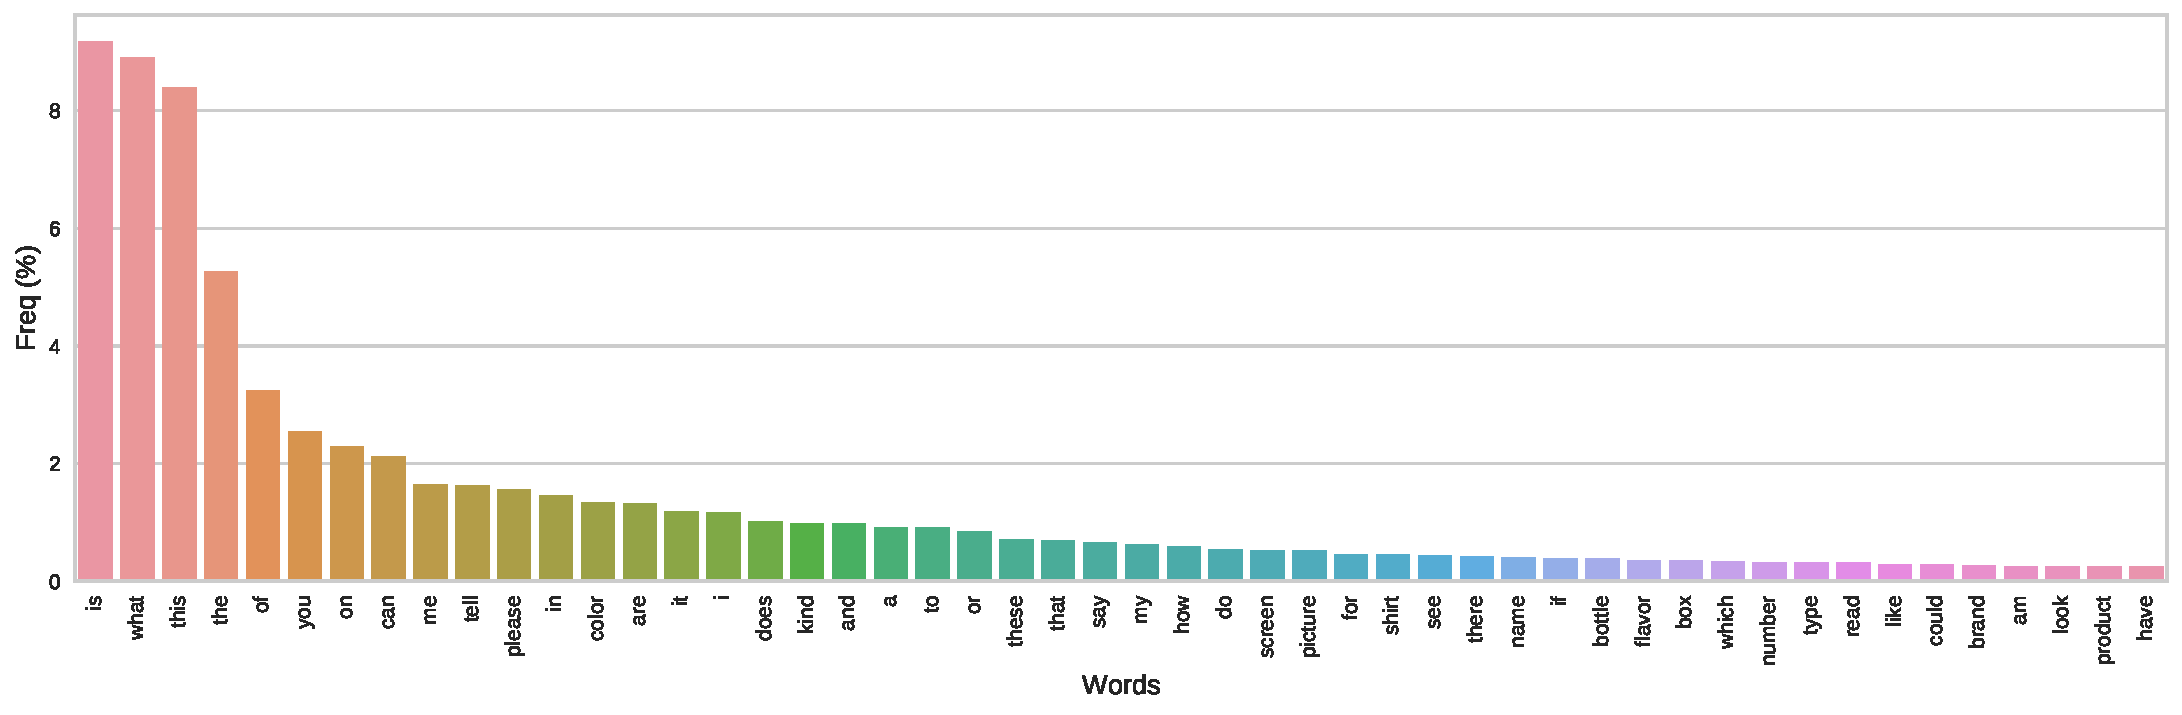
\includegraphics[width=\linewidth]{images/pre/fd_top50_qs_words.pdf}
 \caption{The 50 most frequent words in VizWiz-VQA questions dataset.}
\label{fig:frec_word_qs}
\end{figure*}


\begin{figure}[ht!]
    \centering
    \begin{minipage}[c]{0.49\linewidth}
        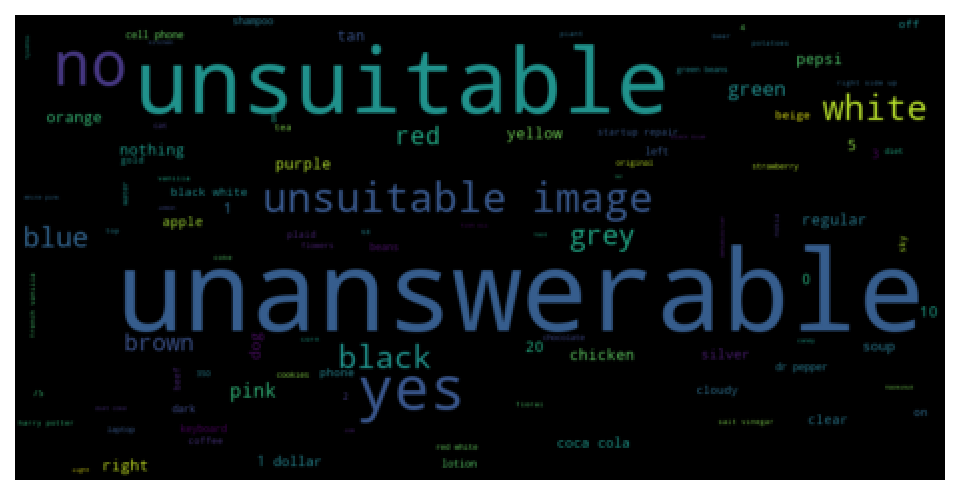
\includegraphics[width=\textwidth]{images/pre/wc_top100_best_ans.pdf}
    \end{minipage}
    %
    \begin{minipage}[c]{0.49\linewidth}
        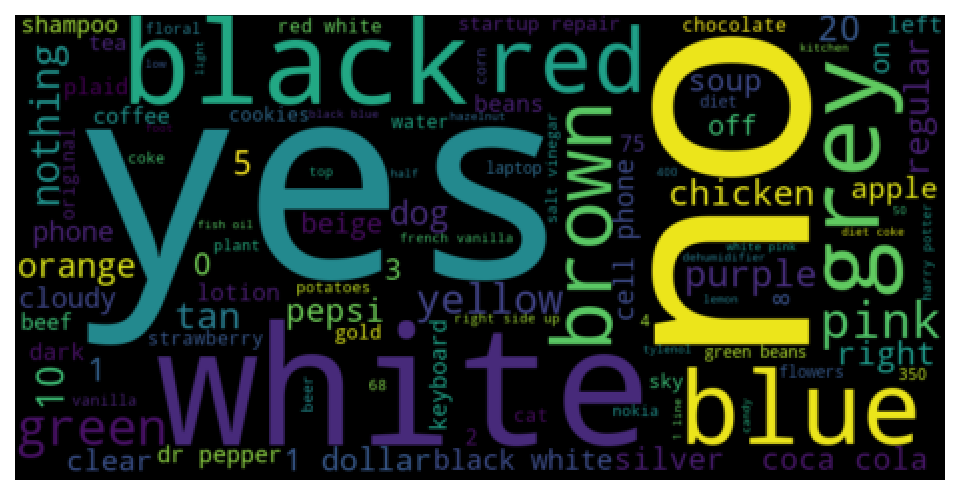
\includegraphics[width=\textwidth]{images/pre/wc_top100_best_ans_red.pdf}
    \end{minipage}
    \caption{The 100 most frequents answers in the VizWiz-VQA dataset. (Left): With 'unsuitable' and `unanswerable' answers. (Right): Without 'unsuitable' and `unanswerable' answers)}
    \label{fig:wc_ans}
\end{figure}

\subsection{Data representations}
% Para la representación de los datos, se utilizaron dos diferentes tipos de embedding: I) embedding basados en matrices de ocurrencia + reducción de dimensionalidad; y II) embedding obtenidos de modelos neuronales pre-entrenados.
For the representation of the data, two different types of embedding were used: I) embedding based on occurrence matrices + dimensionality reduction; and II) embedding obtained from pre-trained neural models.

% Para el primer tipo (I), se testearon distintas combinaciones de concatenaciones de datos de entrada. Mediante el uso de la librería `spacy', se probaron: ``lista de lemas de preguntas'', ``listas de lemas de preguntas + lista de lemas de mejor respuesta'', ``lista de lemas de preguntas + lista de lemas de todas las respuestas''; y de igual  forma con combinaciones de palabras sin lematizar y PoS (Part of speech) de las preguntas. Cabe aclarar que en las concatenaciones resultantes, para poder diferenciar los lemas pertenecientes a las preguntas de los pertenecientes a las respuestas, se añadieron tokens especiales \emph{CLS} y \emph{SEP}, ubicados al inicio y final de cada lista.
For type (I), different combinations of input data concatenations were tested. Using the \emph{spaCy} library, the following were tested: `question lemma list', `question lemma lists + best answer lemma list', `question lemma list + all answer lemma list'; in the same way with combinations of words without stemming and PoS (Part of Speech) of the questions. It should be noted that in the resulting concatenations, in order to differentiate the lemmas belonging to the questions from those belonging to the answers, the special tokens \textbf{CLS} and \textbf{SEP} were added, located at the beginning and end of each list.

% La construcción de las matrices de ocurrencia fueron realizadas utilizando diferentes rangos de n-gramas, desde (1-grama,..,3-grama) hasta un máximo de (1-grama,...,10-gramas). Posterior a esto, se realizó la reducción de dimensionalidad mediante un humbral de varianza. La misma, se implementó a través del método VarianceThreshold de `sklearn', entregando vectores de dimensiones que oscilaron entre 90 y 120.
The construction of the occurrence matrices were performed using different ranges of n-grams, from (1-gram,..,3-gram) to a maximum of (1-gram,...,10-grams). After this, the dimensionality reduction was performed using a variance threshold. It was implemented through the \emph{varianceThreshold} method of the \emph{sklearn} library, providing vectors with dimensions that ranged from 90 to 120.

% Para el segundo tipo de embedding (II), se probaron codificaciones usando modelos pre-entrenados a nivel de palabras, mediante \textbf{fastText}, y a nivel de sentencias, mediante \textbf{doc2Vec}; ambos pertenecientes a la libreria `gensim'. En el caso particular de `fastText', se emplearon dos estrategias en para la obtención del embedding resultante. Por un lado se uso una sumatoria (elemento a elemento), y por el otro una multiplicación, de cada uno de los embedding individuales codificados.
For the type of embedding (II), encodings were tested using pre-trained models at the word level, using \emph{fastText}, and at the sentence level, using \emph{doc2Vec}; both from the \emph{gensim}\footnote{\url{https://pypi.org/project/gensim/}} library. For the particular case of the \emph{fastText} model, two strategies were used to obtain the resulting embedding: summation of individual embedding on the one hand, and multiplication of individual embedding on the other.

\subsection{First approach}
\label{subsec:first_approach}
% Como primera aproximación al problema, se realizaron una sucesión de ejecuciones del algoritmo KMeans, utilizando diferentes rangos de valores de k (k=número de clusteres deseados). La evaluación de resultados fue efectuada de manera visual y cualitativa, ayudándose de la generación de gráficas de Silohuette que guiaron el proceso de selección de los valores k más óptimos. A rasgos generales, en este primer contacto, se busco reducir el conjunto de variables y configuraciones que arrojaran mejores agrupaciones, y conocer el trasfondo del comportamiento de los resultados.
As a first approximation to the problem, a succession of executions of the KMeans algorithm were carried out, using different ranges of k values, where $k=number\_of\_desired\_clusters$. The evaluation of the results was carried out visually and qualitatively, with the help of the generation of Silohuette graphs that guided the selection process of the most optimal k values. In general terms, in this first contact, we sought to reduce the set of variables and configurations that would yield better groupings, and to know the background of the behavior of the results.

% De tales pruebas, se observó que muchas preguntas del estilo: \emph{`please, can you tell me what is in this box?'} y \emph{`what is in this can?'}, eran ubicadas en clusteres diferentes a pesar de poseer semánticas similares. Luego de realizar una revisión detallada del conjunto completo, se identificó que ciertas oraciones de naturaleza conversacional, que precedían a las preguntas, eran las responsables de confundir al algoritmo de clusterización; una lista completa de todas las secuencias identificadas puede ser encontrada en Anexo (). Tal hallazgo, forzó a un nuevo re-procesamiento de datos, y re-generación de listas de `lemas', `PoS' y `tokens' utilizados en la generación de cada embedding. Ahora, cada vez que una sentencia de estas características era identificada como sub-secuencia de una pregunta, sus tokens no eran añadidos a las listas.
% Otro aspecto importante observado, fue que combinaciones de entrada basadas en lista de PoS y palabras sin lematizar, entregaban resultados muchos menos precisos que al usar diferentes combinaciones de listas de lemas.
From such tests, it was observed that many questions like: \ emph {`please can you tell me what's in this box? '} And \ emph {`what's in this can?'}, They were placed in different clusters, despite having similar semantics. After conducting a detailed review of the complete set, it was identified that certain conversational sentences located at the beginning of the questions, were responsible for confusing the grouping algorithm. A complete list of all identified sequences can be found in the Annex (\ref{app:conversational_seq}). This finding forced a new data re-processing, and re-generation of lists of `lemmas', `PoS' and `tokens' used in the generation of each embedding. Now, every time a statement of these characteristics was identified as a sub-sequence of a question, its tokens were not added to the lists.
Another important aspect observed was that input combinations based on Part of Speech lists and non-stemmed words, gave much less accurate results than when using different combinations of lemmas lists.

\subsection{Selection of the best strategy}
\label{subsec:best_strategy}
% Con toda la información obtenida de la primera aproximación, y teniendo en cuenta el objetivo principal de desagregar las categorías mayoritarias de VizWiz-VQA, mediante los grupos de preguntas retornadas por el algoritmo de clusterización; en esta segunda etapa, se incorporaron métodos de testeo mas sistemáticos para poder cuantificar la calidad de los resultados.
With all the information obtained from the first approximation (\ref{subsec:first_approach}), and given the main objective of disaggregating the majority categories of VizWiz-VQA through the groups of questions returned by the clustering algorithm; In this second stage, more systematic testing methods were incorporated in order to quantify the quality of the results.

% Uno de ellos, fue el conocido método de Elbow (o método del codo). Este es un a heurística que se usa para determinar el número de clusters en un conjunto de datos. Este método gráfica la variabilidad como función del número de clusters, y selecciona el `codo' de la curva  como el número de clusters a utilizar. A pesar de que se testearon amplios rangos de valores (entre 3 y 20), todas las curvas obtenidas tenian un comportamiento bastante lineal, por lo que sus resultados no fueron de mucha utilidad.
One of them was the well-known \emph{Elbow} method. This is a heuristic used to determine the number of clusters in a data set. This method graphs the variability as a function of the number of clusters, and selects the `elbow' of the curve as the number of clusters to use. Although wide ranges of values were tested (between 3 and 20), all the curves obtained had a fairly linear behavior, so their results were not very useful.

% Como segundo método de testeo, se confeccionó un conjunto de datos de pruebas, formado de N tuplas de preguntas aleatorias, seleccionadas de entre las 9003 del conjunto de datos filtrados. Se etiqueto cada par con `Si' (`No'), acorde a si las preguntas deberían (o no) pertenecer al mismo cluster.
As a second method, a test dataset was made, made up of N tuples of random questions, selected from among the 9003 of the filtered data set. Each pair was labeled with Yes/No, according to whether the questions should/or not, belong to the same cluster.
% En total fueron anotados 230 pares, y se calcularon los porcentajes de acierto, tanto para aquellos en que la tupla de preguntas caían en un mismo cluster, coincidiendo con la anotación manual, y viceversa para los que no lo hacían.
% A pesar de que esta última estrategia arrojó datos estadísticos muy útiles para la selección de la mejor estrategia, se necesitó de una supervisión humana adicional para  determinar la validez y consistencia de los resultados. Muchos de ellos, a pesar de indicar buenos índices de Silohuette, y altos porcentajes de acierto en el conjunto de datos de prueba, agrupaban preguntas por tipo y morfología, y no por similitud semántica.
In total, 230 pairs were labeled, and the percentages of correct answers were calculated, both for those in which the tuple of questions fell into the same cluster, coinciding with the manual annotation, and vice versa for those who did not.
Although the latter method yielded very useful data for selecting the best strategy, additional human supervision was required to determine the validity and consistency of the results. Many of them, despite indicating good Silohuette indices, and high accuracy percentages  in the test dataset, grouped questions by type and morphology, and not by semantic similarity.

% En total, dejando de lado las pruebas realizadas en la primera aproximación, se exploraron nueve estrategias de clusterización diferentes (resultados en Tabla \ref{table:strategies_results}). La selección final fué realizada buscando un equilibrio entre calidad/consistencia de clusteres entregados, y porcentajes de aciertos en el conjunto de datos de prueba confeccionado.
In total, leaving aside the tests carried out in the first approximation, nine different clustering strategies were explored (see Table (\ref{table:strategies_results})). The final selection was made looking for a balance between quality/consistency of clusters delivered, and percentages of correct answers in the set of test data prepared.

\begin{table*}[!th]
	\centering
	\scalebox{.9}{
	\begin{tabular}{c | c | c| c | c | c | c | c}
		\toprule
		\textbf{Data Input} & \textbf{N-grams} & \textbf{Min\_df}  & \textbf{Var Threshold} & \textbf{Embedding}   & \textbf{Best K}      & \textbf{Same cluster}     & \textbf{Diff cluster}     \\ \midrule
		Qsl                         & 1,3-grams           & 10          & .01           & 117         & 8           & 47.54\%          & 91.41\%          \\
		Qst+QsPoS+BestAns           & 1,10-grams          & 10          & .001          & 97          & 19          & 36.07\%          & 94.4\%           \\
		\textbf{Qst+BestAns}        & \textbf{1,10-grams} & \textbf{10} & \textbf{.001} & \textbf{99} & \textbf{17} & \textbf{44.26}\% & \textbf{99.39}\% \\
		Qst+BestAns (w/ Noun mask)  & 1,7-grams           & 10          & .001          & 113         & 17          & 47.5\%           & 96.9\%           \\
		Qst+AllAns                  & 1,3-grams           & 10          & .001          & 74          & 25          & 26.23\%          & 96.9\%           \\
		Qst+BestAns (Doc2Vec)       & 4-grams             & 1           & -             & 100         & 18          & 14.7\%           & 87.7\%           \\
		Qst+AllAns (Doc2Vec)        & 4-grams             & 1           & -             & 100         & 14          & 29.5\%           & 90.8\%           \\
		Qst+AllAns (FastText-vSum)  & 4-grams             & 1           & -             & 100         & 21          & 13.1\%           & 97.5\%           \\
		Qst+AllAns (FastText-vMult) & 4-grams             & 1           & -             & 100         & 16          & 24.5\%           & 87.7\%     \\      
		\bottomrule
	\end{tabular}}
	\caption{Results and metrics of clustering strategies. (Qsl): List of question lemmas - 
		(Qst): List of question words without lemmatize -
		(WsPoS): List of question's Part of speech -
		(BestAns): List of lemmas of answer with most agreement -
	(AllAns): List of lemmas of all answers from question.}
	\label{table:strategies_results}
\end{table*}

\paragraph{\textbf{Best strategy}}. 
% La estrategia final seleccionada entregó \textbf{17} clusteres de preguntas (ver Anexo()). Las Figuras (\ref{fig:silohuette}) y (\ref{fig:clustering2d}), muestran el nivel de consistencia `gráfico de Silhouette', y la distribución aproximada, T-SNE de por medio, visualizadas en un gráfico de dos dimensiones. \footnote{Si bien la identificación de los clusteres de la Figura (\ref{fig:clustering2d}) se corresponde con Anexo(), la misma podría no ser directa en el gráfico de Silohuette (Figura \ref{fig:silohuette}), ya su generación fue realizada por separado.}
The final strategy selected delivered \textbf{17} question clusters, see Annex (\ref{app:clusters}). Figures (\ref{fig:silohuette}) and (\ref{fig:clustering2d}), show the consistency level `Silhouette graph', and the approximate distribution respectively. The second, after the application of T-SNE\footnote{\url{https://en.wikipedia.org/wiki/T-distributed_stochastic_neighbor_embedding}}, to be visualized in a two-dimensional graph.\footnote{Although the identification of the clusters in the Figure (\ref{fig:clustering2d}) corresponds to the indices of the clusters described in Annex (\ref{app:clusters}), the same correspondence might not be direct in the Silohuette graph in Figure (\ref{fig:silohuette}), since its generation was carried out separately.}


\begin{figure}[ht!]
    \centering
    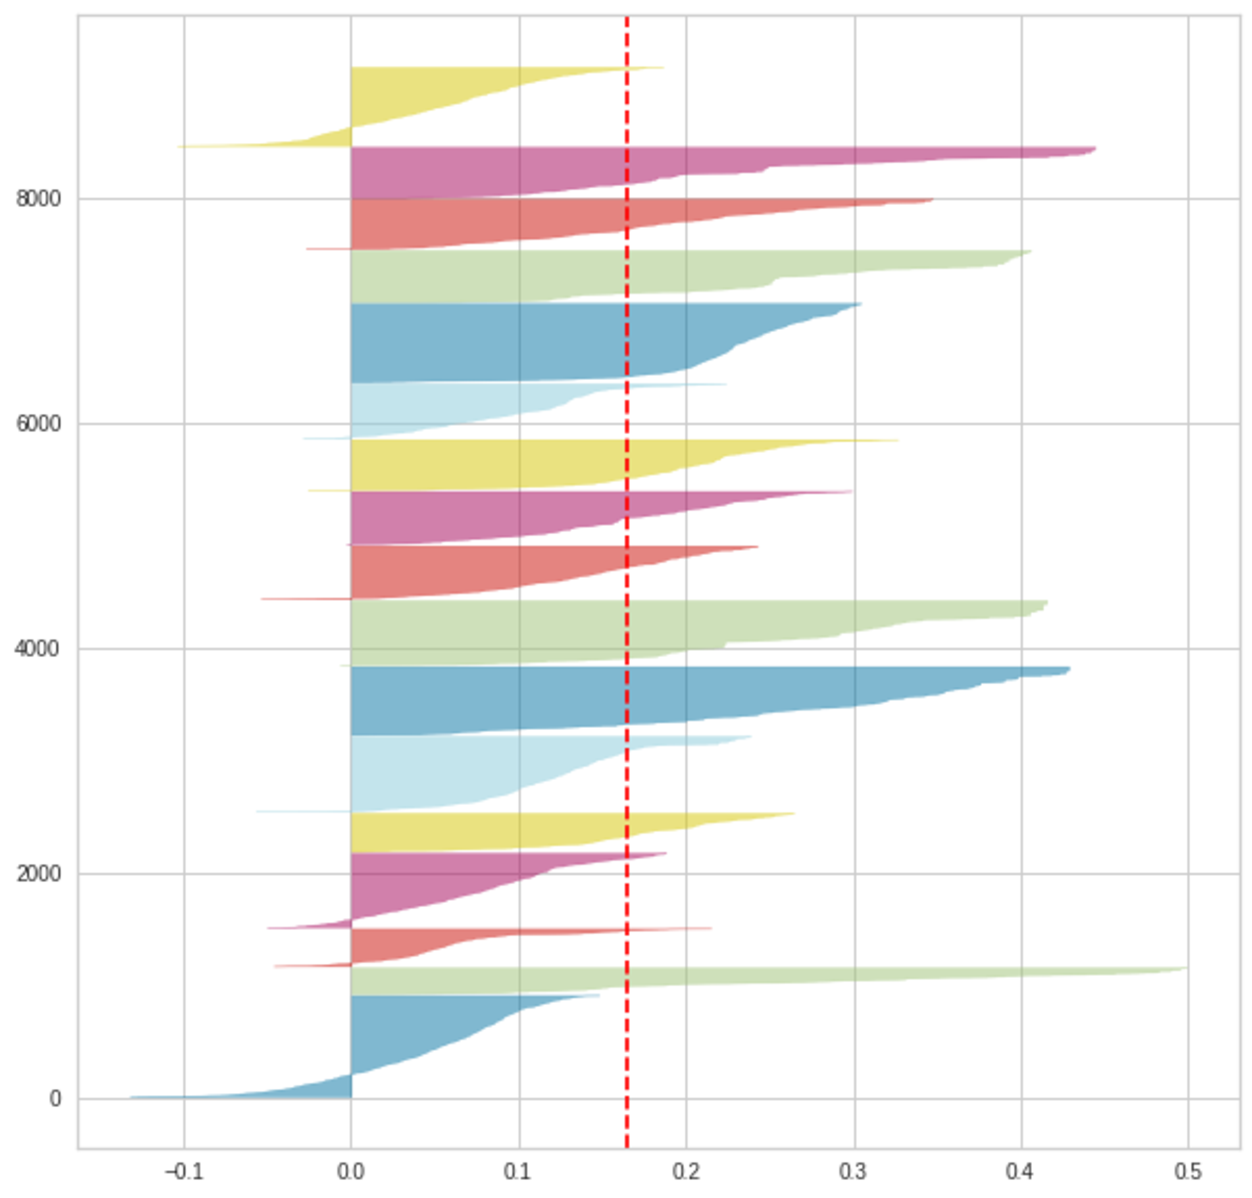
\includegraphics[width=\linewidth]{images/pre/silhouette_opc2_clustering.pdf}
\caption{Clusters consistency, through Silhouette scores.}
\label{fig:silohuette}
\end{figure}

\begin{figure}[ht!]
    \centering
    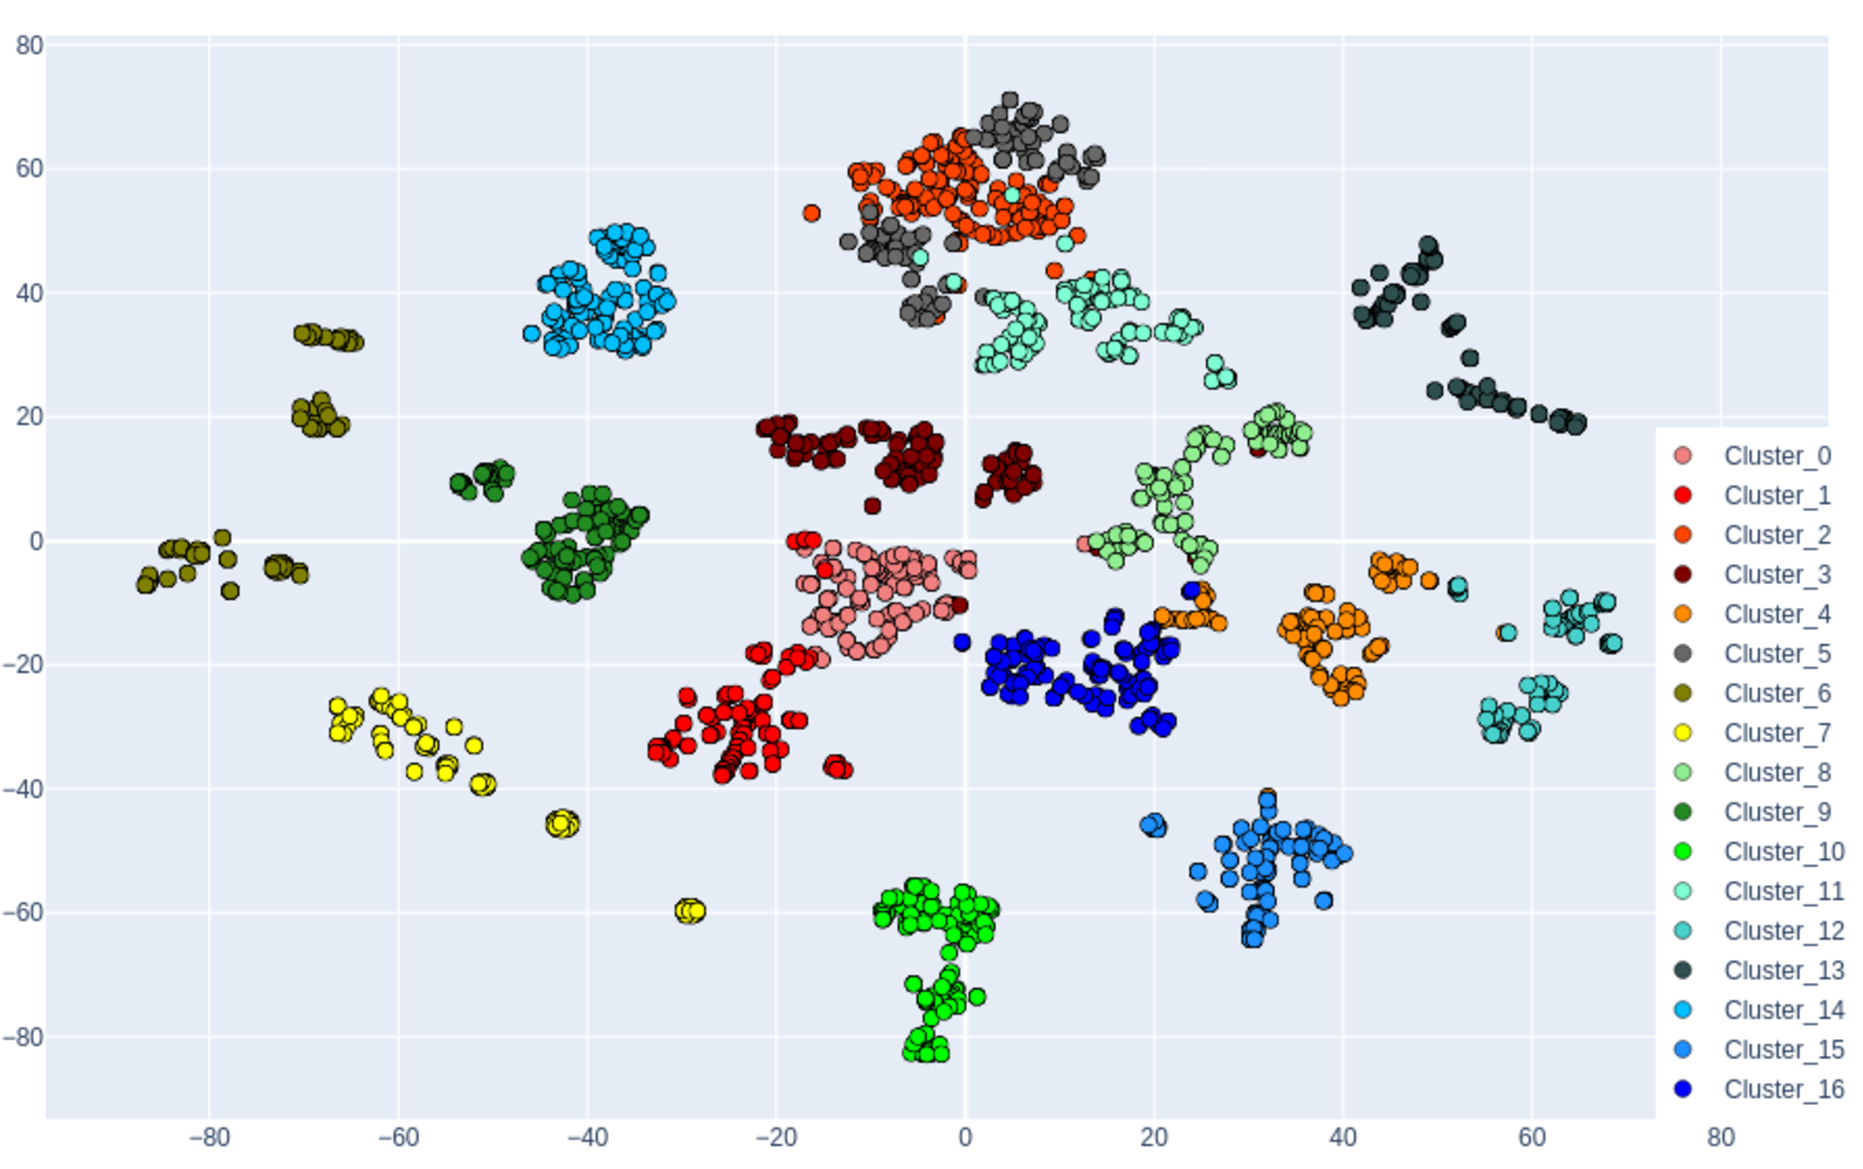
\includegraphics[width=\linewidth]{images/pre/plot2d_opc2_clustering.pdf}
\caption{Clusters distributions, displayed through T-SNE method.}
\label{fig:clustering2d}
\end{figure}


% Con respecto a los datos de entrada, esos resultaron de la concatenación de las listas de: \textbf{``lemas de pregunta + lemas de mejor respuesta''}; mientras que los embedding que alimentaron al algoritmo de Kmeans, se basaron en una matriz de ocurrencia con \textbf{1-gramas,...,10-gramas} como columnas de características. Una posterior reducción de dimensionalidad mediante umbral de varianza, descartó columnas de características con variaciones menores al \textbf{.001}, produjendo vectores finales de dimensionalidad \textbf{99}.
% Esta estrategia además, otorgó un \textbf{44.26\%} de precisión en las tuplas de control anotadas como pertenecientes a clusters similares, y un \textbf{99.33\%} para las anotadas como pertenecientes a clusters diferentes (Figura (\ref{fig:metrics})).
Regarding the input data, these resulted from the concatenation of the lists of: \textbf{`question lemmas + best answer lemmas'}; while the embeddings that fed the Kmeans algorithm were based on an occurrence matrix with \textbf{1-grams, ..., 10-grams} as feature columns, with a subsequent dimensionality reduction, using the technique of variance threshold, which discarded columns of characteristics with variations less than \textbf{.001}, producing final vectors with a dimensionality of \textbf{99}.
This strategy also gave a \textbf{44.26\%} precision in the control tuples annotated as belonging to similar clusters, and a \textbf{99.33\%} for those annotated as belonging to different clusters (Figure (\ref{fig:metrics})).

\begin{figure}[ht!]
    \centering
    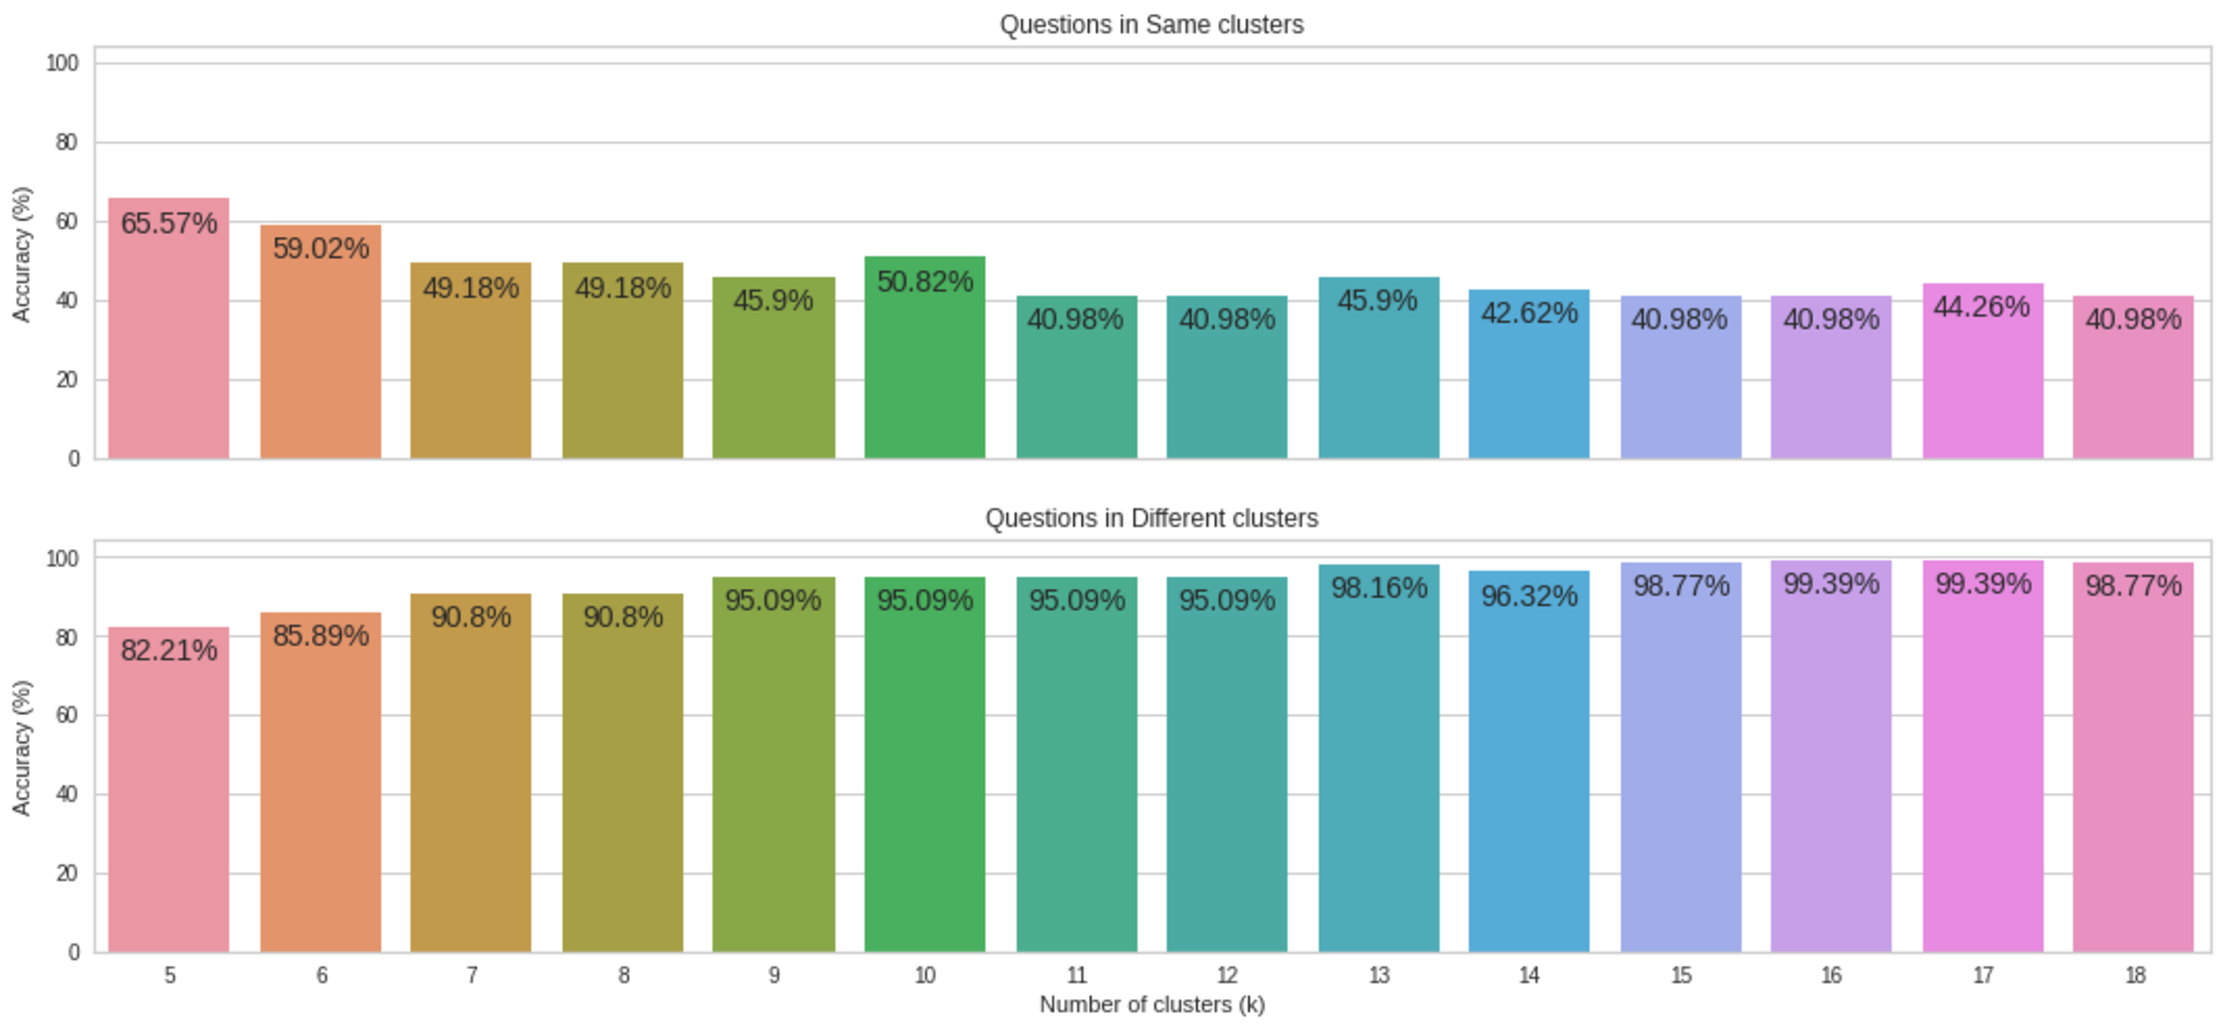
\includegraphics[width=\linewidth]{images/pre/metricts_opc2_clustering.pdf}
    \caption{Percentages of accuracy of the tuples considered to belong to the same clusters, and those considered to belong to different clusters, in relation to the results returned by the `KMeans' algorithm using a given k value.}
\label{fig:metrics}
\end{figure}

% En función de los resultados y experimentos realizados, se observó que las estrategias de clusterización basadas en embedding de tipo II fueron mucho mas ineficientes que las basadas en matrices de ocurrencia para algun rango de n-gramas. Tal observación, puede ser atribuida a la relativa poca cantidad de datos utilizados para la generación de los embedding, sumado a que los modelos utilizados no fueron pre-entrenados en conjuntos de datos de naturaleza conversacional.
% Por otro lado, los mejores rendimientos fueron alcanzados con datos de entrada construidos por concatenación de tokens de preguntas y respuestas lematizados. El aporte de respuesta con menos coincidencia generaron efectos negativos.
% Con respecto al la calidad de los clusteres, se notó que a medida que las preguntas se alejan de los centroides (ganan mayor distancia), se va perdiendo algo de consistencia. En linea general, se obtuvieron conjuntos de preguntas que comparten una mayor similitud morfológica que semántica, y están medianamente influenciados por sus respuestas. A pesar de ello, clusters como $0$, $1$, $5$ y $15$ resultaron de gran calidad y pureza, y combinaciones como $12$ y $13$, $16$ y $4$, entre otros, pudieron ser caracterizadas de manera muy precisa.
Based on the results and experiments carried out, it was observed that the clustering strategies based on type II embedding were much more inefficient than those based on occurrence matrices for some range of n-grams. Such observation can be attributed to the relative small amount of data used for the generation of the embedding, added to the fact that the models used were not pre-trained in datasets of a conversational nature.
On the other hand, the best performances were achieved using as input data, a concatenation of the question and answer lemma lists. It was also observed that the inclusion of answers with fewer coincidences produced a negative effect.
Regarding the quality of the clusters, it was noted that as the questions move away from the centroids (they gain greater distance), some consistency is lost. In general, sets of questions were obtained that share greater morphological than semantic similarity, and are moderately influenced by their answers. Despite this, clusters such as $0$, $1$, $5$ and $15$ were of great quality and purity, and combinations such as $12$ and $13$, $16$ and $4$, could be characterized very precisely.
\section{Classifier}
\label{sec:classifier}
% El objetivo principal de entrenar un clasificador utilizando los clusteres de preguntas obtenidas en la Sección (), fue lograr la desagregación de los grupos mayoritarios de VizWiz-VQA, mediante la propuesta de nuevas categorias detalladas en Subsección ().
% La Subsección (), describe el proceso de entrenamiento para los diferentes modelos de clasificación entrenados. La Subsección (), testea aquellos con mayores precisiones, y contrasta sobre el conjunto total de datos de VizWiz-VQA, las antiguas categorizaciones, de las nuevas retornadas por los modelos.
The main objective of training a classifier using the clusters of questions obtained in Subsection (\ref{subsec:best_strategy}), was to achieve the disaggregation of the majority groups of VizWiz-VQA, by proposing new categories detailed in Subsection (\ref{subsec:categories_assignment}).
Subsection (\ref{subsec:training_models}), describes the training process for the different trained classification models. Later in Section (\ref{sec:models_testing}), the most accurate models will be tested and contrasted on the total set of VizWiz-VQA data, the old categorizations, of the new classes returned by the models.

\subsection{Categories assignment}
\label{subsec:categories_assignment}
% Si bien la mayoría de las agrupaciones encontradas en la Sección () ya tenian cierta coherencia, el algoritmo de KMeans realizó la separación de conjuntos basándose tambien en las respuestas, quedando por ejemplo preguntas cerradas respondidas con `yes' por un lado, y respondidas con `No' por el otro. Es por esto, que no se alimentará directamente al modelo de clasificacion con el contenido de cada cluster, sino que se realizará un paso previo de refinamiento.
Although most of the groupings found in Subsection (\ref{subsec:best_strategy}) already had some coherence, the KMeans algorithm also performed the separation of sets based on the answers, leaving, for example, closed questions answered with `yes' on the one hand, and answered with 'no' for the other. This is why the classification model will not be fed directly with the content of each cluster, without first performing a previous refinement step.

% Para la caracterización y/o definición de las nuevas clases, primero se identificaron los clusters más puras, es decir, aquellas agrupaciones que solamente contenian un tipo particular de preguntas, cualquiera fuesen sus respuestas; por ejemplo: colores, identificación de objetos, preguntas con opciones, preguntas cerradas, etc. Luego, entre los clusters restantes, se buscaron características compartidas que pudieran agrupar y ser representativas para dos, tres o mas de ellos.
For the characterization and/or definition of the new classes, first the purest clusters were identified, that is, those groupings that only contained a particular type of questions, without considering their answers, for example: colors, identification of objects, questions with options, closed questions. Then, among the remaining clusters, shared characteristics were searched that could group and be representative for two, three or more of them.

% Como resultado, se definieron 8 nuevas clases, capaces de representar de manera natural a 15 de los 17 agrupaciones analizados. Dada su variada composición, los clusters restantes (7 y 9 de Anexo()), fueron dejados de lado, para evitar introducir errores en el proceso de entrenamiento del modelo de clasificación. Los siguientes items, describen y ejemplifican las nuevas clases propuestas:
As a result, \textbf{8 new classes} were defined, capable of representing in a natural way 15 of the 17 analyzed groups. Given their varied composition, the remaining clusters (7 and 9 of Annex (\ref{app:clusters})), were left aside, to avoid introducing errors in the training process of the classification model. The following items describe and exemplify the new proposed classes:

\begin{itemize}
    \item \textbf{c0) color}. Color identification: Questions asked with the intention of obtaining information about the color of a certain object. \emph{e.g:
        'what colors is my jeans?',
        'what is the color for this laptop?',
        'which color has the purse?',
        'what color is my t-shirt please?'}
    
    \item \textbf{c1) ocr}. Need for ocr: Questions directly aimed at obtaining specific information (textual or numerical) that helps to complete the identification of a previously identified object. e.g: \emph{
    'what is the name of this film?',
    'what is the expiration date of this almond milk?',
    'what is the title of this disc?',
    'what is the phone model?'}
    
    \item \textbf{c2) observation}. Observations: Questions where the person needs to know an appreciation or obtain textual or visual information of some characteristic of an object or scene in order to be informed. \emph{e.g:
    'what does this box say on top?',
    'this is sky look like?',
    'what does this computer screen say?',
    'what does this pregnancy test show?'}
    
    \item \textbf{c3) ident}. Direct identification: Direct question for the identification of an object, or some property or characteristic that allows to finish identifying it. e.g: \emph{
    'what is this recipe?',
    'what brand of earbuds are these?',
    'what kind of battery is this?',
    'coffee is this?',
    'what type of tile is this?'}
    
    \item \textbf{c4) rel\_ident}. Relative identification: Object identification question, through referential descriptions that involve already located or known objects. e.g: \emph{
    'can you see what is in this package?',
    'what is on my shelves?',
    'what is inside this?',
    'what is written in screen?',
    'what is inside this canned good?'}
    
    
    \item \textbf{c5) explication}. Complex answer questions: Questions with several objectives, whose formulation of the answer requires knowledge of what is being asked or involves giving location instructions, recognizing people or giving an explanation of a random topic. e.g:\emph{ 
    'where is this made?',
    'who is this dog?',
    'why is this computer not booting up?',
    'where is this box from?',
    'who is this mail for?',
    'where you thinking about this one?'}
    
    
    \item \textbf{c6) choice}. Choice selection: Questions where the answer is explicit in the question, and one of the listed options must be returned. e.g: \emph{
    'is this iphone or nokia?',
    'is this blue or purple?',
    'is this decaf or regular coffee?',
    'is this brown rice or white rice?'}
    
    
    \item \textbf{c7) yes\_no}. Confirmations: Status questions. Binary response (yes/no).  e.g:. \emph{
    'is this the new apple keyboard?',
    'are those piano keys?',
    'is this the blue?',
    'is this an iphone?',
    'is my light off?',
    'is he fat?',
    'see anything?'}

\end{itemize}

\subsection{Training}
\label{subsec:training_models}
% Antes de comenzar a entrenar los modelos de clasificación, se identificaron y etiquetaron las peguntas de cada clusters con las nuevas clases propuestas, see Table (\ref{table:clusters_assigned}). 
Before starting to train the classification models, the questions of each cluster were identified and labeled with the new proposed classes, see Table (\ref{table:clusters_assigned}).

\begin{table}[!ht]
    \centering
    \begin{tabular}{l|c|r}
        \toprule
        \textbf{Ref} &\textbf{Class} &\textbf{Clusters assigned} \\ \midrule
        c0 & color & [0] \\
        c1 & ocr & [16,3] \\
        c2 & observation & [1]\\
        c3 & ident & [2,8,11,6]\\
        c4 & rel\_ident & [14]\\
        c5 & explication & [4,10,15]\\
        c6 & choice & [5]\\
        c7 & yes\_no & [12,13] \\
        \bottomrule
    \end{tabular}
    \caption{Classes proposed and cluster assignations.}
    \label{table:clusters_assigned}
\end{table}

% Para entrenar cada uno, se tomaron las primeras $N$ preguntas más cercanas al centroide del cluster al que pertenecían. En el caso de las clases asignadas a un número de clusters $C >= 2$, se tomaron las primeras  $\floor{N/C}$ preguntas de cada uno, para conseguir un dataset de entrenamiento balanceado. Esta cantidad, se definió individualmente según los resultados arrojados en cada modelo entrenado, tomando como $N$ definitivo, aquel valor que mayor precisión entregara en el grupo de testeo.
To train each one, the first $N$ questions closest to the centroid of the cluster to which they belonged were taken. In the case of the classes assigned to a number of clusters $C >= 2$, the first $\floor{N / C}$ questions of each one were taken, to obtain a balanced training dataset. This amount was defined individually according to the results obtained in each trained model, taking as the final $N$, the value that delivered the highest precision in the testing group.

% Con la intención de que el modelo de clasificación pudiese categorizar cualquier tipo de pregunta, se descartó entrenar el modelo re-utilizando los embedding creados en el proceso de clusterizació, ya que ante la llegada de una pregunta por fuera del grupo usado para entrenamiento o testeo, no podría obtenerse su representación característica.
% Como consecuencia, se optó por codificar las preguntas con dos modelos de embedding neuronales pre-entrenados: \emph{bert\_base\_uncased} \footnote{\url{https://huggingface.co/bert-base-uncased}} y \emph{all-MiniLM-L6-v2} \footnote{\url{https://huggingface.co/sentence-transformers/all-MiniLM-L6-v2}}; ambos en el estado del arte.
% % , incluidos en la librería \emph{sentenceTransformer} \footnote{\url{https://www.sbert.net/}}
With the intention that the classification model could categorize any type of question, training the model re-using the embedding created in the clustering process was discarded, since upon the arrival of a question outside the group used for training or testing , its characteristic representation could not be obtained.
As a consequence, it was decided to encode the questions with two pre-trained neural embedding models: \emph{bert\_base\_uncased}\footnote{\url{https://huggingface.co/bert-base-uncased}} and \emph{all-MiniLM-L6-v2}\footnote {\url{https://huggingface.co/sentence-transformers/all-MiniLM-L6-v2}}; both in the state of the art.

% Para el proceso de tipificación de preguntas, se pusieron a prueba los clasificadores \emph{LogisticRegresion} y  \emph{Linear Suport Vector Classification (LinearSVC)}; utilizando una división 80/20 del conjunto de datos, para el entrenamiento y testeo de las 4 combinaciones resultantes. Las Figuras (\ref{fig:m1}), (\ref{fig:m2}), (\ref{fig:m3}) y (\ref{fig:m4}) muestran, matrices de confusión, porcentajes de precisión y valores de $N$ utilizados, para las combinaciones \textbf{M1}: \emph{`bert\_base\_uncased + LogisticRegression'}, \textbf{M2}: \emph{`bert\_base\_uncased + LinearSVC'}, \textbf{M3}: \emph{`all-MiniLM-L6-v2 + LogisticRegression'} y \textbf{M4}: \emph{`all-MiniLM-L6-v2 + LinearSVC'} respectivamente.
For the question typing process, the classifiers \emph{Logistic Regression} and \emph{Linear Suport Vector Classification (LinearSVC)} were tested; using an 80/20 division of the data set to train and test the resulting 4 combinations. The Figures (\ref{fig:m1}), (\ref{fig:m2}), (\ref{fig:m3}) and (\ref{fig:m4}) show confusion matrices, precision percentages and the $N$ values used, for the combinations: \textbf{M1}: \emph{`bert\_base\_uncased + Logistic Regression'}, \textbf{M2}: \emph{`bert\_base\_uncased + LinearSVC '}, \textbf{M3}: \emph{`all-MiniLM-L6-v2 + Logistic Regression'} and \textbf{M4}: \emph{`all-MiniLM-L6-v2 + LinearSVC'} respectively.


\begin{figure}[ht!]
    \centering
    \begin{minipage}[c]{0.49\linewidth}
        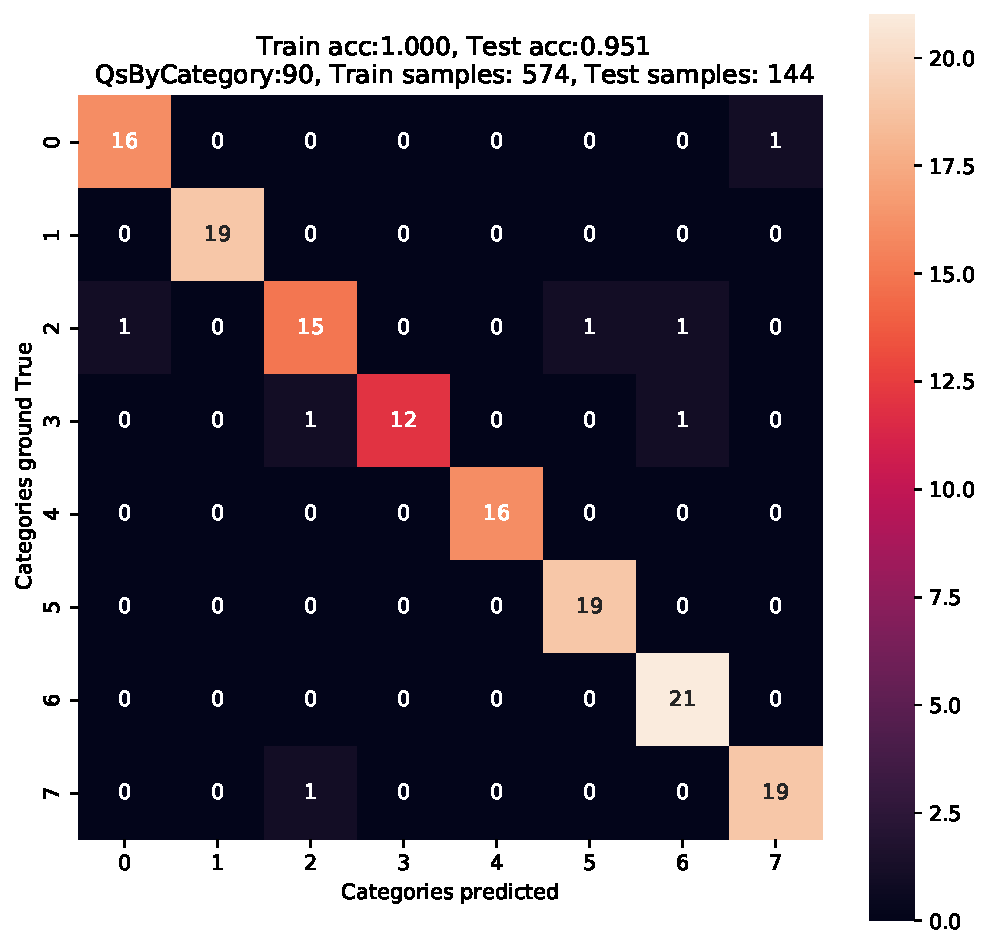
\includegraphics[width=\textwidth]{images/training/training_m1_v2.pdf}
        \caption{Training results of M1: `bert\_base\_uncased + Logistic Regression'.}
        \label{fig:m1}
    \end{minipage}
    %
    \begin{minipage}[c]{0.49\linewidth}
        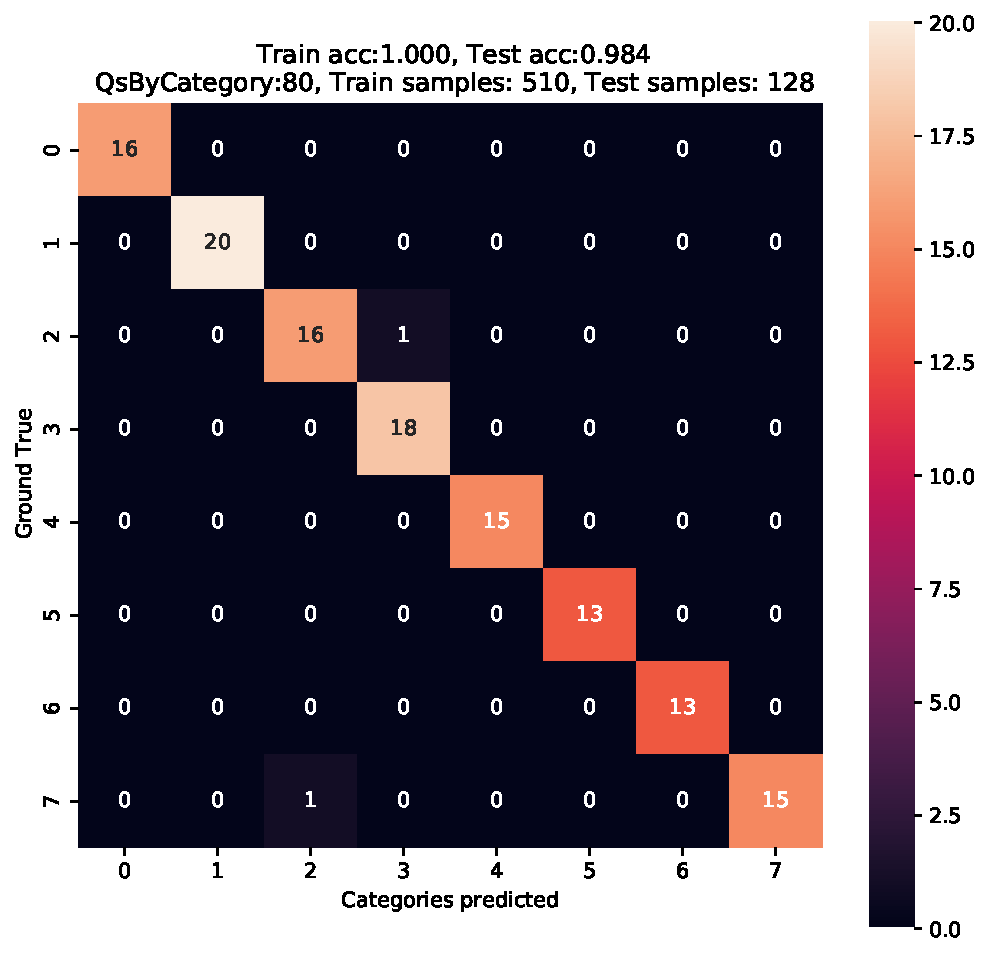
\includegraphics[width=\textwidth]{images/training/training_m2_v2.pdf}
        \caption{Training results of M2: `bert\_base\_uncased + LinearSVC'.}
        \label{fig:m2}
    \end{minipage}
\end{figure}

\begin{figure}[ht!]
    \centering
    \begin{minipage}[c]{0.49\linewidth}
        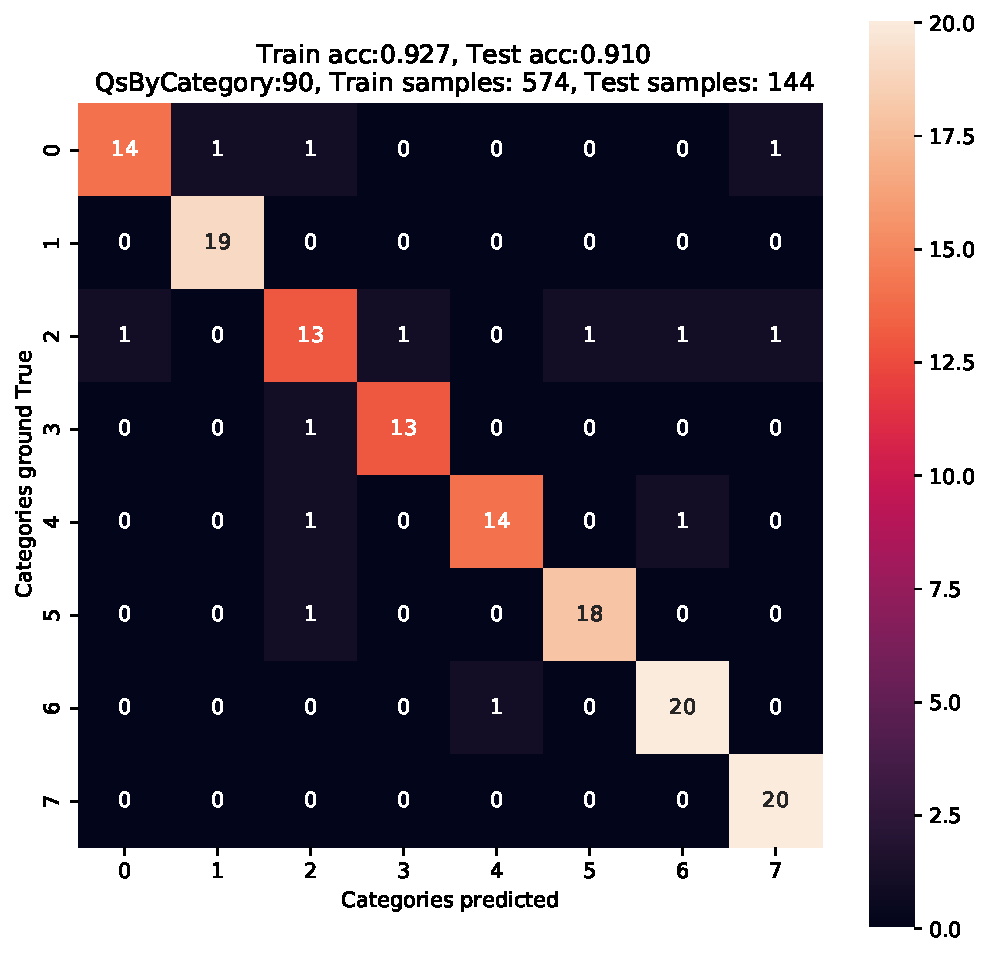
\includegraphics[width=\textwidth]{images/training/training_m3_v2.pdf}
        \caption{Training results of M3: `all-MiniLM-L6-v2 + Logistic Regression'.}
        \label{fig:m3}
    \end{minipage}
    %
    \begin{minipage}[c]{0.49\linewidth}
        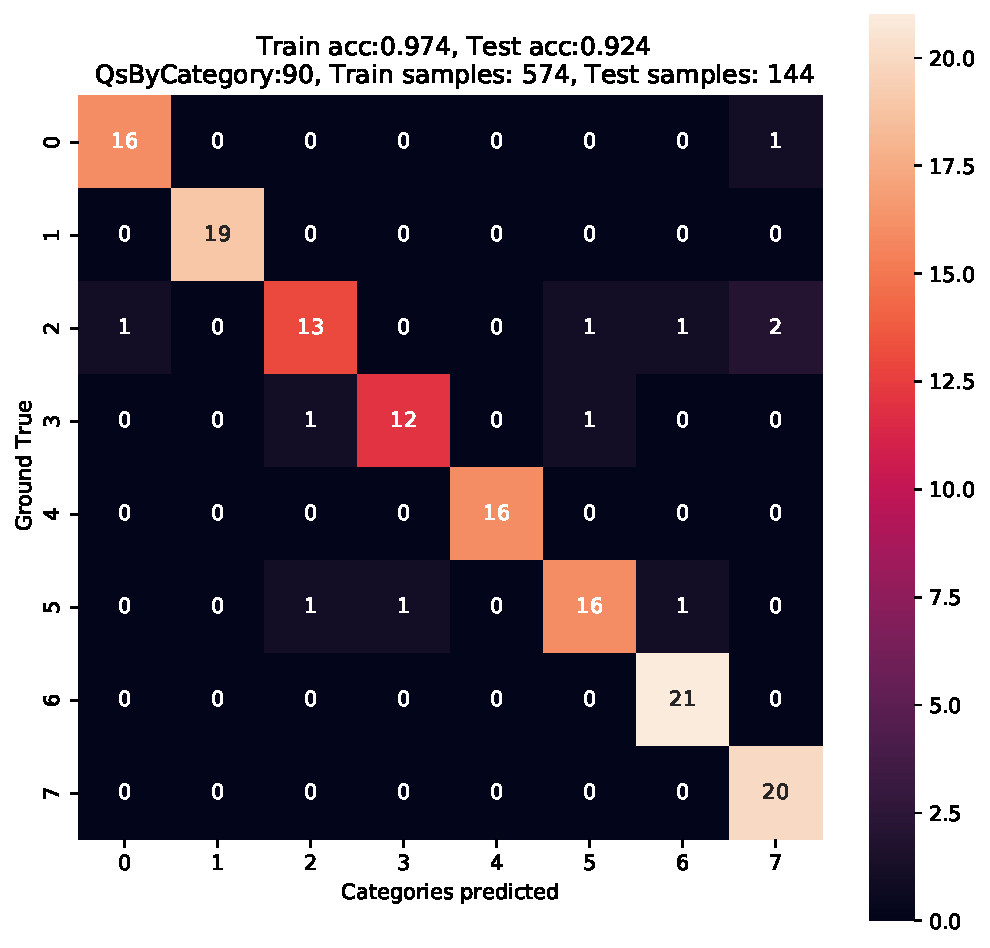
\includegraphics[width=\textwidth]{images/training/training_m4_v2.pdf}
        \caption{Training results of M4: `all-MiniLM-L6-v2 + LinearSVC'.}
        \label{fig:m4}
    \end{minipage}
\end{figure}

% Teniendo en cuenta los resultados anteriores, si bien las cuatro combinaciones lograron buenas precisiones, se observa un leve incremento de rendimiento en aquellas combinaciones que utilizaron \emph{LinearSVC} como modelo de clasificación multi-clase. Por otro lado, al comparar rendimientos en relación a modelos de embedding empleados, las codificaciones con \emph{bert\_base\_uncased } fueron superiores. Esto último, pudiendose atribuir a la mayor cantidad de información contenida en los vectores de dimensionalidad $768$ generados, contra $384$ para \emph{all-MiniLM-L6-v2}. La Figura (\ref{fig:dist_m2}), muestra la distribución de predicciones sobre todas las preguntas de los 17 clusters analizados, utilizando la combinación M2.
Taking into account the previous results, although the four combinations achieved good precision, a slight increase in performance is observed in those combinations that used \emph{LinearSVC} as a multi-class classification model. On the other hand, when comparing performances in relation to the embedding models used, the encodings with \emph{bert\_base\_uncased} were superior. The latter, being attributable to the greater amount of information contained in the generated dimensionality vectors $768$, against $384$ for \emph{all-MiniLM-L6-v2}. The Figure (\ref{fig:dist_m2}), shows the distribution of predictions on all the questions of the 17 analyzed clusters, using the M2 combination.


\begin{figure}[ht!]
    \centering
    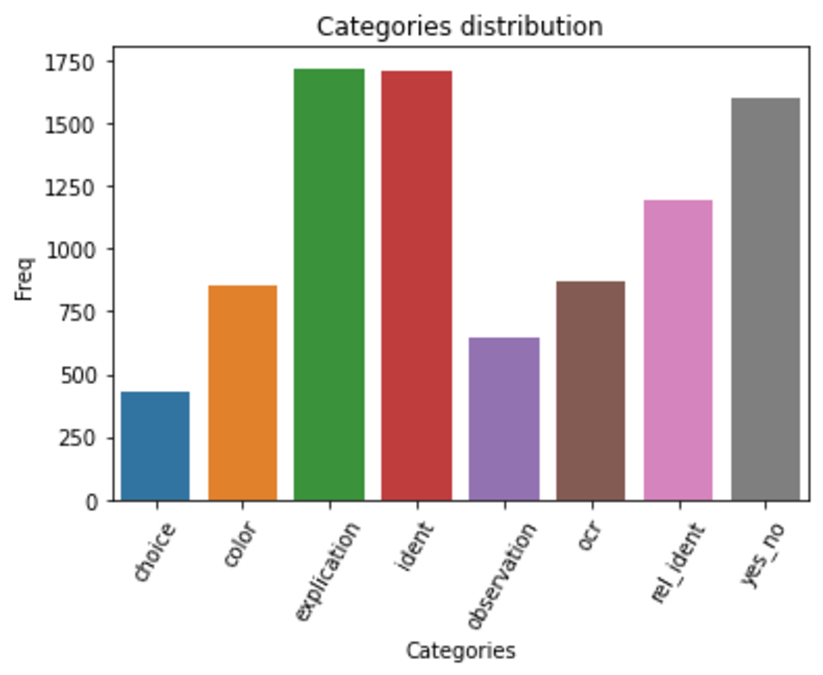
\includegraphics[width=.9\linewidth]{images/training/distribution_m2_v2.pdf}
\caption{Categories distribution using predictions of the models combination M2.}
\label{fig:dist_m2}
\end{figure}
\section{Models testing}
\label{sec:models_testing}
% En esta última sección, se analizarán los resultados de las predicciones obtenidas utilizando la combinación M2 (bert\_base\_uncased + LinearSVC), que fue la que en terminos generales, con un $\sim$ 100\% para el grupo de entrenamiento y un 98\% para el grupo de testeo, entrego las mejores precisiones. A diferencia de la sección anterior (Sección ), en donde se generaron distribuciones de predicciones sobre las 9003 preguntas pre-procesadas (Subsección ), en esta etapa, el modelo será alimentado con el total de preguntas del conjunto de datos VizWiz-VQA sin filtrar. Nuevamente, el conjunto de testeo será dejado a un lado, ya que no posee respuestas asociadas y por ende categorías para poder contrastar resultados.
In this last section, the results of the predictions obtained using the M2 combination (bert\_base\_uncased + LinearSVC) will be analyzed, which was the one that in general terms, with 98\% precision in the testing group, delivered the best results. Unlike the previous section, Section (\ref{sec:classifier}), where prediction distributions were generated on the 9003 pre-processed questions, Figure (\ref{fig:dist_m2}); at this stage, the model was fed with all questions from the unfiltered VizWiz-VQA dataset. Again, the test set will be left aside, since it does not have associated answers and therefore categories to be able to contrast results.

% La Figura (\ref{fig:mco_mod2}), muestra la matriz de confusión entre las nuevas clases: 
% \emph{choice}, \emph{color}, \emph{explication}, \emph{ident}, \emph{observation}, \emph{ocr}, \emph{rel\_ident}, \emph{yes\_no}, y las antiguas categorías: \emph{yes/no, unanswerable, other, number}; sobre el total de 24842 preguntas. Notar que cada celda de la matriz, representa que porcentaje de la antigua categoria ('answer\_type') fué clasificada con la predicción indicada inmediatamente debajo, sobre el eje horizontal.
Figure (\ref{fig:mco_mod2}), shows the confusion matrix between the new classes:
\emph{choice}, \emph{color}, \emph{explanation}, \emph{ident}, \emph{observation}, \emph{ocr}, \emph{rel\_ident}, \emph{yes\_no }, and the old categories: \emph {yes/no, unanswerable, other, number}; over the total of 24842 questions. Note that each cell of the matrix represents what percentage of the old category ('Answer Type') was classified with the prediction indicated immediately below, on the horizontal axis.

\begin{figure}[ht!]
    \centering
    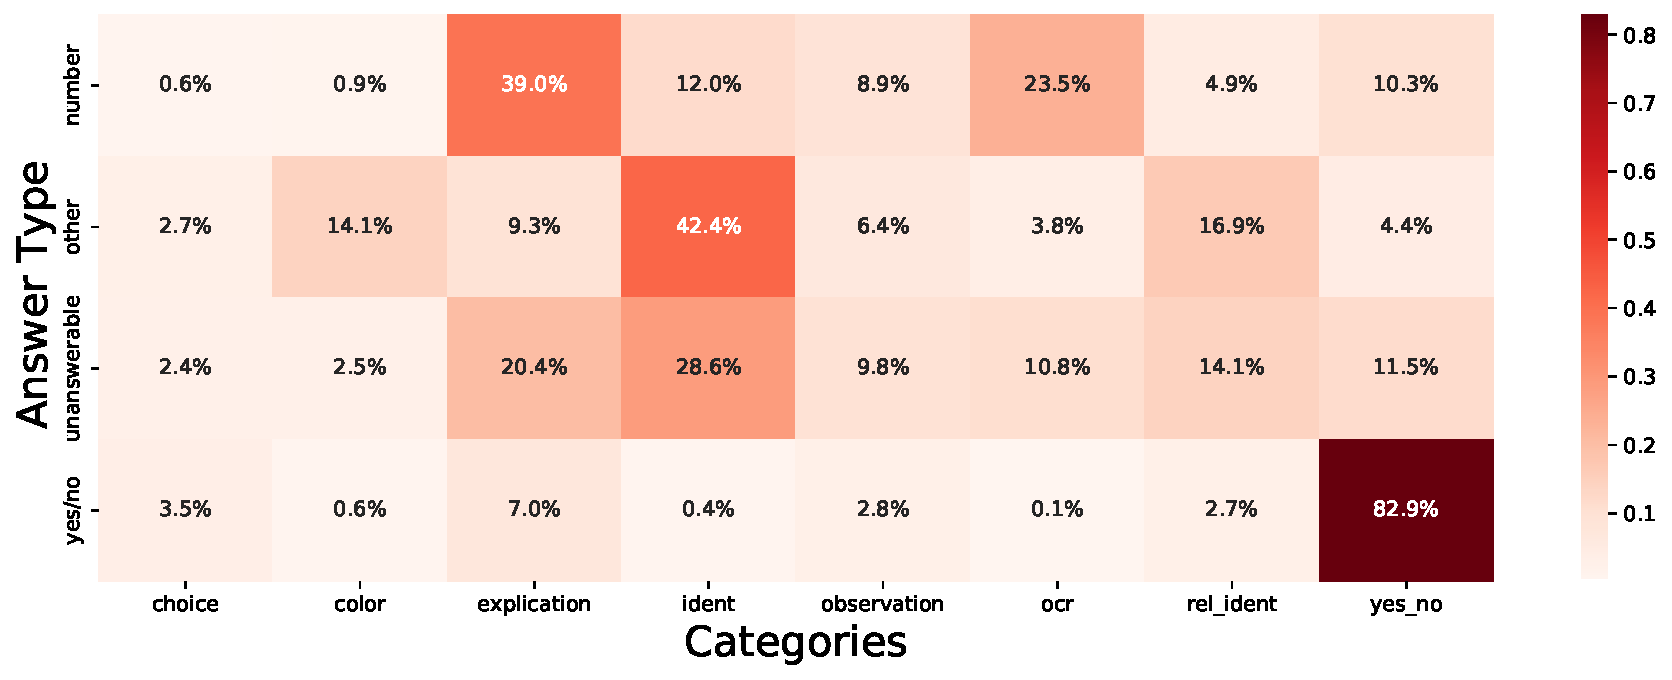
\includegraphics[width=\linewidth]{images/testing/mc_m2_v2.pdf}
\caption{Confusion matrix of M2 combination: 'bert\_base\_uncased + LinearSVC', over full VizWiz-VQA dataset.}
\label{fig:mco_mod2}
\end{figure}


% Dos observaciones naturales que inicialmente se pueden realizar sobre la matriz de la Figura (), son sobre las clases 'number' y 'yes/no'; únicas clases originales descriptivas del conjunto. 
% Si miramos la clase 'yes/no', podemos ver que el $\sim$82\% de las preguntas mantuvieron su categorización, lo que da una muy buena primera impresión, respecto de la confianza de nuestro clasificador.
% Al analizar la clase 'number', vemos que las predicciones se centran con el $\sim$23\% y el $\sim$39\% en las predicciones 'ocr' y 'explication' respectivamente. A pesar de que pueda a primera vista parecer erróneo, esto es muy consistente, ya preguntas del tipo: \emph{'How many cups are there?', How many doors? or 'How many fingers in this image?'} requieren contar objetos, y no necesitan capacidades de reconocimiento optico de caracteres como: \emph{'What is the number on this barcode?', 'What is the oven temperature setting?' or 'What is the second number?'}.
Two natural observations that can initially be made on the matrix of Figure (\ref{fig:mco_mod2}), are on the classes 'number' and 'yes/no'; unique descriptive original classes of the set. If we look at the 'yes/no' class, we can see that the $\sim$82\% of the questions maintained their categorization, which gives a very good first impression, regarding the confidence of our classifier.
When analyzing the class 'number', we see that the predictions are centered with the $\sim$23\% and the $\sim$39\% in the predictions `ocr' and `explication' respectively. Although it may seem wrong at first glance, this is quite consistent. Questions such as: \emph{`How many cups are there?', `How many doors?' or `How many fingers in this image?'} require counting objects, and do not need optical character recognition capabilities such as: \emph{`What is the number on this barcode?', `What is the oven temperature setting?' or `What is the second number?'}.

% Poder descubrir la conformación de la clase 'other', fue una de las principales motivaciones que llevaron a desarrollar este trabajo. Se pueden ver tres grandes sub-clases que la caracterizan: 'color', 'rel\_ident' y 'ident' con el $\sim$14\%, $\sim$16\% y $\sim$42\% respectivamente. Lo cual indica que en esta clase se mezclan preguntas de identificación de colores e identificaciones de objetos directos como indirectos, mediante características o propiedades ya conocidas. Algunos ejemplos de tales grupos se detallan en Tabla (\ref{table:res_other}). 
Being able to discover the conformation of the 'other' class was one of the main motivations that led to develop this work. You can see three large sub-classes that characterize it: `color', `rel\_ident' and `ident' with the $\sim$14\%, $\sim$16\% and $\sim $42\% respectively. Which indicates that this class mixes questions of identification of colors and identifications of direct and indirect objects, through characteristics or properties already known. Some examples of such groups are detailed in Table (\ref{table:res_other}).


\begin{table}[!th]
    \centering
    \scalebox{0.80}{
        \begin{tabular}{l|c|r}
            \toprule
            \textbf{Answer Type} & \textbf{Category} & \textbf{Question} \\ \midrule
            other         & ident      & What kind of soup is this? \\
            other         & ident      & What are these? \\
            other         & ident      & What is this product? \\
            other         & ident      & What kind of pie is this? \\ \midrule
            other         & rel\_ident  & What is in this jar? \\
            other         & rel\_ident  & what is in front of me? \\
            other         & rel\_ident  & What is against the wall next to the door? \\
            other         & rel\_ident  & What is on this package? \\ \midrule
            other         & color      & Is my shirt dirty and what color is it? \\
            other         & color      & What color is this cover? Thank you \\
            other         & color      & What color are my pants? \\
            other         & color      & What is the color for this keyboard? \\
            other         & color      & What color is this? \\
        \bottomrule
        \end{tabular}}
        \caption{Examples of predictions for old class `other'.}
        \label{table:res_other}
\end{table}

% Por último, al analizar la clase 'unanswerable', se observa que las predicciones con mayores porcentajes se corresponden a 'explication', 'yes\_no' y nuevamente 'ident' y 'rel\_ident'. Cuatro categorías que requieren de una imagen asociada bien definida y en contexto con la pregunta realizada, para que puedan ser correctamente contestadas; algo que no caracteriza a este dataset.

% En Anexo (), se detallan 50 predicciones aleatoria, realizadas con los modelos de la combinacion M2, sobre el conjunto de datos VizWiz-VQA.
Finally, when analyzing the class `unanswerable', it is observed that the predictions with the highest percentages correspond to `explication', `yes\_no' and again `ident' and `rel\_ident'. Four categories that require a well-defined associated image and in context with the question asked, so that they can be correctly answered; something that does not characterize this dataset.

In Annex (\ref{app:classification_samples}), 50 random predictions samples are detailed with each of eight new categories, made with the models of the M2 combination, on the VizWiz-VQA dataset.
\section{Conclusions and Future directions}
% El esfuerzo principal de este trabajo fue destinado a obtener una desagregación de las clases mayoritarias del conjunto de preguntas a respuestas visuales VizWiz-VQA. 
% En una primera etapa, se emplearon técnicas no supervisadas y distintas estrategias de codificación de datos de entrada, con el fin de  alimentar al algorítmo de clusterización con el embedding que mejores resultados entregara. En esta parte, se utilizo el algoritmo KMeans como método de clusterización, y dos estrategias de embedding: una basada en construcción de matrices de ocurrencia mediante n-gramas + reducción de dimensionalid, y la otra, mediante modelos pre-entrenados de embedding neuronales, tales como fastText y doc2Vec.
The main effort of this work was aimed at obtaining a disaggregation of the majority classes of the set of visual questions VizWiz-VQA.
In a first stage, unsupervised techniques and different input data coding strategies were used, in order to feed the clustering algorithm with the embedding that would deliver the best results. In this part, the \emph{KMeans} algorithm was used as a clustering method, and two embedding strategies: one based on the construction of occurrence matrices through n-grams + dimensionalid reduction, and the other, through pre-trained neural embedding models. such as \emph{fastText} and \emph{doc2Vec}.

% Posterior a la clusterización, se inició un proceso de análisis de resultados en busca de propiedades y catracterísticas que permitieran identificar naturalmente cada uno de los clusteres obtenidos. Como consecuencia, se propuso un conjunto de 8 nuevas categorias: \textbf{choice, color, explanation, ident, observation, ocr, rel\_ident, yes\_no}, sentando las bases para el desarrollo de la segunda fase del proyecto. El objetivo de la identificación de nuevas clases para sustituir las ya predefinidas en el conjunto de datos originales, se debió a que estas últimas, son inespecificas y no permiten conocer en profundidad el tipo y naturaleza de preguntas que contienen.
After the clustering, a process of analysis of the results was started in search of properties and characteristics that would allow the natural identification of each one of the clusters obtained. As a consequence, a set of 8 new categories was proposed: \emph{choice, color, explanation, ident, observation, ocr, rel\_ident, yes\_no}, laying the foundations for the development of the second phase of the project. The objective of identifying new classes to replace those already predefined in the original dataset was due to the fact that the latter are unspecific and do not allow in-depth knowledge of the type and nature of questions they contain.

% Con las nuevas clases ya definidas, en la segunda estapa, se entrenaron dos modelos de clasificadores: Logistic Regression y Linear Suport Vector CLassification. Además, con la finalidad de que el modelo final fuera capaz de etiquetar a cualquier pregunta por fuera de los grupos de entrenamiento y testeo utilizados, los datos de entrada para tal entrenamiento (en este caso, las preguntas), fueron codificados probando dos modelos pre-entrenados de embedding neuronales, ámbos en el estado del arte: bert\_base\_uncased y all-MiniLM-L6-v2. Como resultado, luego de poner a prueba cuatro combinaciones (modelo de embedding, modelo de clasificación), se seleccionó a la tupla (bert\_base\_uncased, LinearSVC) como modelo definitifo, entregando $\sim$98\% de precisión en el conjunto de preguntas de testeo.
With the new classes already defined, in the second stage, two classifier models were trained: \emph{Logistic Regression} and \emph{Linear Suport Vector Classification}. In addition, in order for the final model to be able to label any question outside of the training and testing groups used, the input data for such training (in this case, the questions) were coded by testing two pre-trained models of neural embedding, both in the state of the art: \emph{bert\_base\_uncased} and \emph{all-MiniLM-L6-v2}. As a result, after testing four combinations (embedding model, classification model), the tuple \emph{bert\_base\_uncased + LinearSVC} was selected as the definitive model, giving $\sim$ 98\% precision in the set of test questions.

% Posteriormente, con el modelo de clasificación entrenado sobre las nuevas categorías de preguntas propuestas, se pudo realizar el esperado desagregado del conjunto completo de VizWiz-VQA. Los resultados obtenidos al etiquetar todas las preguntas con las nuevas 8 clases, permitieron conocer varios puntos importantes. 
Subsequently, with the classification model trained on the new proposed question categories, the expected disaggregation of the complete set of VizWiz-VQA could be carried out. The results obtained when labeling all the questions with the new 8 classes, allowed to know several important points.

% Las antiguas clases `yes/no' y `number', fueron las dos categorizaciones mas puras encontradas. Para la primera, casi el 83\% de las respuestas eran binarias. Por otro lasdo, en la clase `number' se observó que no solo habia preguntas relacionadas directamente al reconocimiento de números en algun entorno dado, sino que  también, preguntas relacionadas a conteos de objetos formaban el $\sim$39\% del grupo y no requerían de capacidades OCR.
% Con respecto a las clases más emblemáticas, en `other' las preguntas caian principalmente dentro de tres subcategorías, siendo las relacionadas con la identificación de objetos la destacada, seguida por preguntas de tipo relacionales y por último de identificación de colores.Para el caso de `unanswereable', se identificaron cuatro tipos de predicciones principales: `explication', `ident', `rel\_ident', `yes\_no'. De estas, las tres primeras son categorías de preguntas muy dificiles de responder ya que requieren capacidades de razonamiento, conocimientos previos y manejo de la perspectiva muy grandes; si a esto se le suma las caracterizticas malas calidades de las imágenes asociadas, no sería una sorpresa que este tipo de preguntas ocupen esta misteriosa clasificación.
The old classes `yes/no' and `number', were the two purest categorizations found. For the first one, almost 83\% of the answers were binary. On the other hand, in the class `number' it was observed that not only were there questions directly related to the recognition of numbers in some given environment, but also, questions related to object counts made up $\sim$ 39\% of the group and not required OCR capabilities.
With respect to the most emblematic classes, in `other' the questions fell mainly into three subcategories, those related to the identification of objects being the most prominent, followed by relational questions and finally color identification. For the case of `unanswerable', four main types of predictions were identified: `explication', `ident', `rel\_ident' and `yes\_no'. Of these, the first three are categories of questions that are very difficult to answer since they require very great reasoning skills, prior knowledge and management of perspective; if to this is added the characteristic poor qualities of the associated images, it would not be a surprise that these types of questions occupy this mysterious classification.


% Para finalizar, y pensando en posibles trabajos futuros, se planean utilizar los resultados del modelo de clasificación para entrenar un modelo de preguntas y respuestas condicionado (cQ\&A). Es decir, con las preguntas re-clasificadas, se alimentara el nuevo modelo, no solo con la pregunta de interes, sino con un condicionamiento extra, su categoría. De esta forma, y al igual que lo hacen los algoritmos cGAN (Conditional Generative Adversarial Networks), se podra diriguir el resultado. Esto, es muy interesante ya que preguntas del estilo \emph{`Could you tell me what color is this?'}, que trivialmente serían respondidas con si/no, al pasarle por ejemplo la categoría  `color', se forzaría al modelo para que con suerte, devolviera como respuesta el nombre de un color,  desambiguando la pregunta para recibir el típo específico de respuesta que se desee.
Finally, and thinking about possible future work, it is planned to use the results of the classification model to train a conditioned question and answer model (cQ\&A). That is, with the re-classified questions, the new model will be fed, not only with the question of interest, but also with an extra conditioning, its category. In this way, and as the cGANs \cite{cGans} (Conditional Generative Adversarial Networks) algorithms do, the result can be directed. This is very interesting since questions of the style \emph{`Could you tell me what color is this?'}, which would trivially be answered with yes|no, when passing for example the category `color', the model would be forced to hopefully it will return the name of a color, disambiguating the question to receive the specific type of response that is desired.


\bibliographystyle{splncs04}
\bibliography{biblio}
\nocite{*}

\clearpage
\appendix
% \onecolumn

\section{List of conversational sequences}
\label{app:conversational_seq}
\emph{'can you tell me', 'can you tell', 'tell me', 'please tell me', 'please read', 'can you please tell me',  'please can you tell me', 'could you please tell me', 'can you please', 'can you read to me',  'can you please read', 'can you see','can you read','can you give me','can you help me','are you able to', 'i do not know if this', 'i want to know the'}. 

\section{Top 20 questions from each cluster, from best strategy selected (Qst+BestAns).}
\label{app:clusters}

% \twocolumn
\begin{table}[!th]
	\centering
	\scalebox{0.70}{
		\begin{tabular}{lcr}
			\toprule
			\textbf{Question}               & \textbf{Best Answer} & \textbf{Distance} \\ \midrule
			what color are those pants?     & pink                 & 0.213182          \\
			what color is cup?              & yellow               & 0.230284          \\
			>what color is this product?    & pink                 & 0.237367          \\
			what color is this item?        & grey                 & 0.242185          \\
			what color is this device?      & silver               & 0.248018          \\
			what color is this phone case?  & brown                & 0.248018          \\
			what color is this image?       & blue                 & 0.248018          \\
			what color is this woman's top? & blue                 & 0.254964          \\
			what color is this object?      & green                & 0.254964          \\
			what color is this button?      & clear yellow         & 0.254964          \\
			what color is this table?       & brown                & 0.254964          \\
			what color is this cup?         & blue                 & 0.254964          \\
			what color is this dog?         & brown                & 0.254964          \\
			what color is this gift bag?    & pink                 & 0.254964          \\
			what color is this man's pants. & grey                 & 0.254964          \\
			what color is my book bag?      & blue grey            & 0.262036          \\
			what color is this top ?        & pink                 & 0.263126          \\
			what color is this glass?       & blue                 & 0.263126          \\
			what color is this case?        & green                & 0.263126          \\
			what color is this pant?        & red                  & 0.263126          \\
			\bottomrule
		\end{tabular}}
	\caption{[Cluster 0] --- 20 top questions}
	\vspace{-5mm}
\end{table}

\begin{table}[!th]
	\centering
	\scalebox{0.70}{
		\begin{tabular}{lcr}
			\toprule
			\textbf{Question}                   & \textbf{Best Answer} & \textbf{Distance} \\ \midrule
			what does this cup say.             & 1 3 cup              & 0.241263          \\
			what does this label say?           & green pigeon         & 0.248653          \\
			what does this box look like?       & phone                & 0.257584          \\
			what does this plant look like?     & plant                & 0.261638          \\
			what does this dress look like?     & curtain              & 0.266728          \\
			what does this item look like?      & necklace             & 0.266728          \\
			what does this say                  & intel pentium        & 0.267346          \\
			what does this packet say?          & hot cocoa mix        & 0.267346          \\
			what does this say?                 & 8                    & 0.267346          \\
			what does this box say?             & toad training        & 0.267346          \\
			what does this cup look like?       & movie poster         & 0.272992          \\
			what does the label say?            & shiner rye           & 0.27753           \\
			what does this food label say?      & uncle bens           & 0.278919          \\
			what does this character say?       & 3                    & 0.278919          \\
			what does this label say.           & new bothwell mb      & 0.278919          \\
			what does this box say on top?      & mary kay             & 0.280023          \\
			what does this pregnancy test show? & 1 line               & 0.280586          \\
			what does this monitor look like?   & blank                & 0.280586          \\
			what does he look like?             & dog                  & 0.281864          \\
			what does the sky look like?        & dark                 & 0.282237          \\
			\bottomrule
		\end{tabular}}
	\caption{[Cluster 1] --- 20 top questions}
	\vspace{-5mm}
\end{table}


\begin{table}[!th]
	\centering
	\scalebox{0.70}{
		\begin{tabular}{lcr}
			\toprule
			\textbf{Question}                & \textbf{Best Answer} & \textbf{Distance} \\ \midrule
			what is this item?               & solar garden light   & 0.137387          \\
			what is this wine?               & wine                 & 0.137387          \\
			what is this canned good?        & green beans          & 0.137584          \\
			what is this device?             & cell phone           & 0.137584          \\
			what is this bag look like       & suitcase             & 0.137584          \\
			what is this drink?              & coca cola            & 0.13922           \\
			please tell me what is this box? & 2 spicy bean burgers & 0.13922           \\
			what is this thing right here?   & pepperoni pizza      & 0.140246          \\
			what is this box                 & mcdonalds            & 0.140246          \\
			what is this product key?        & 021 08454            & 0.140246          \\
			what is this soda called?        & pepsi                & 0.140246          \\
			what is this bill?               & 10                   & 0.140246          \\
			what is this label?              & hunts pasta sauce    & 0.140246          \\
			what is this box?                & coconut sponge       & 0.140246          \\
			what is this box from?           & powerskin            & 0.140246          \\
			what is this person wearing?     & blue shorts          & 0.140246          \\
			what is this ready meal package? & chicken              & 0.140246          \\
			what is this spice?              & apple pie spice      & 0.142654          \\
			what is this cup?                & coffee               & 0.145769          \\
			what is this pink packet         & sweet n low          & 0.145769          \\
			\bottomrule
		\end{tabular}}
	\caption{[Cluster 2] --- 20 top questions}
	\vspace{-5mm}
\end{table}

\begin{table}[!th]
	\centering
	\scalebox{0.70}{\centering
		\begin{tabular}{lcr}
			\toprule
			\textbf{Question}                           & \textbf{Best Answer}   & \textbf{Distance} \\\midrule
			what is the sky look like today?            & clear                  & 0.190297          \\
			what is the oven temperature set at?        & 230                    & 0.191961          \\
			what is the brand name?                     & clover organic farms   & 0.194766          \\
			what is the temperature set at?             & 75                     & 0.198866          \\
			what is the oven temperature control setup? & dial                   & 0.204423          \\
			what is the oven control temperature?       & 350                    & 0.211605          \\
			what is the oven temperatures setting?      & 325                    & 0.211605          \\
			what is the name of ths product             & oxibooster             & 0.212719          \\
			what is the sodium content?                 & 10 mg                  & 0.220584          \\
			what is the product?                        & cheese sticks          & 0.220584          \\
			what is the dial set at?                    & 450                    & 0.220584          \\
			what is the name of the mouse brand?        & microsoft              & 0.22708           \\
			what is the name of the cd                  & patsy cline            & 0.22708           \\
			what is the name of the water?              & naturliches            & 0.227491          \\
			what is the name of the drink?              & irn bru                & 0.227491          \\
			what is the name of the story?              & sleep book             & 0.227491          \\
			what is the name of the flower?             & carnation              & 0.227491          \\
			what is the name of the magazine?           & popular mechanics      & 0.228351          \\
			what is the name of the restaurant?         & aladdin natural eatery & 0.229712          \\
			\bottomrule
		\end{tabular}}
	\caption{[Cluster 3] --- 20 top questions}
	\vspace{-5mm}
\end{table}

\begin{table}[!th]
	\centering
	\scalebox{0.70}{
		\begin{tabular}{lcr}
			\toprule
			\textbf{Question}                             & \textbf{Best Answer} & \textbf{Distance} \\ \midrule
			can you read who this christmas card is from? & unanswerable         & 0.216867          \\
			where is this box from?                       & unanswerable         & 0.221511          \\
			what food is inside this packet?              & unanswerable         & 0.225636          \\
			where is this nut from?                       & unanswerable         & 0.230656          \\
			where is this coin from                       & unanswerable         & 0.230656          \\
			what temperature is this dial set too?        & unanswerable         & 0.231024          \\
			who is this parcel from?                      & unanswerable         & 0.237108          \\
			where is this from?                           & unanswerable         & 0.237108          \\
			when is this card?                            & unanswerable         & 0.237108          \\
			who is this from?                             & unanswerable         & 0.237108          \\
			what size is this item?                       & unanswerable         & 0.237371          \\
			where is this table?                          & unanswerable         & 0.245022          \\
			who is this dog?                              & unanswerable         & 0.245022          \\
			why is this computer not booting up?          & unanswerable         & 0.254572          \\
			who is this person?                           & unanswerable         & 0.254572          \\
			what temperature is this thermostat set to?   & unanswerable         & 0.260985          \\
			what size of cereal is this box.              & unanswerable         & 0.262043          \\
			what temperature is this oven set to          & unanswerable         & 0.263272          \\
			who is this character?                        & unanswerable         & 0.265953          \\
			where is this made?                           & unanswerable         & 0.265953          \\
			\bottomrule
		\end{tabular}}
	\caption{[Cluster 4] --- 20 top questions}
	\vspace{-5mm}
\end{table}

\begin{table}[!th]
	\centering
	\scalebox{0.70}{
		\begin{tabular}{lcr}
			\toprule
			\textbf{Question}                              & \textbf{Best Answer} & \textbf{Distance} \\ \midrule
			is this candy or chocolate?                    & chocolate            & 0.196788          \\
			is this regular or decaf coffee?               & regular              & 0.196788          \\
			is this fire engine red or yellow              & red                  & 0.196788          \\
			is this blue or purple?                        & blue                 & 0.19726           \\
			is this regular or caffeine free?              & caffeine free        & 0.19726           \\
			is this regular mountain dew or diet?          & regular              & 0.19726           \\
			is this shower gel or lotion?                  & gel                  & 0.19726           \\
			is this catalina regular or catalina free?     & free                 & 0.19726           \\
			is this sweatshirt brown or tan?               & brown                & 0.19726           \\
			is this diet or regular pepsi?                 & diet                 & 0.19726           \\
			is this diet pepsi, regular, or caffeine free? & diet                 & 0.19726           \\
			is this cloth pink or blue?                    & pink                 & 0.19726           \\
			is this flowers or stripes?                    & stripes              & 0.19726           \\
			is this yarn blue or purple?                   & purple               & 0.197804          \\
			is this stripes or flowers?                    & flowers              & 0.197804          \\
			is this shampoo, conditioner, or lotion?       & conditioner          & 0.197804          \\
			is this decaf or regular coffee?               & regular              & 0.197804          \\
			is this shampoo or conditioner?                & shampoo              & 0.197804          \\
			is this with chocolate or with fruit?          & chocolate            & 0.197804          \\
			is this inhaler blue or yellow?                & yellow               & 0.197804          \\
			\bottomrule
		\end{tabular}}
	\caption{[Cluster 5] --- 20 top questions}
	\vspace{-5mm}
\end{table}

\begin{table}[!th]
	\centering
	\scalebox{0.70}{
		\begin{tabular}{lcr}
			\toprule
			\textbf{Question}               & \textbf{Best Answer}    & \textbf{Distance} \\ \midrule
			what dollar bill is this?       & 5                       & 0.165812          \\
			what denomination is this?      & 20                      & 0.165812          \\
			what temperature is this?       & 450                     & 0.16603           \\
			what brand is this>             & trojan                  & 0.16603           \\
			what brand is this?             & winston                 & 0.16603           \\
			what schwan's dinner is this?   & beef shepherds pie      & 0.167918          \\
			what harry potter book is this? & sorcerers stone         & 0.167918          \\
			what bill is this?              & 1 dollar                & 0.168106          \\
			what product is this?           & cereal almonds          & 0.17162           \\
			what bill denomination is this? & 1 dollar                & 0.17162           \\
			what dollar amount is this?     & 5                       & 0.172827          \\
			what dinner is this?            & beef strips             & 0.172827          \\
			what card is this?              & justice                 & 0.172827          \\
			what video game is this?        & tiger woods pga tour 10 & 0.172827          \\
			what gift card is this?         & dunkin donuts           & 0.172827          \\
			what gift card is this          & tim hortons             & 0.172827          \\
			what cleaning product is this?  & 409 all purpose cleaner & 0.172827          \\
			what food is this?              & pizza                   & 0.172827          \\
			what product is this            & coffee                  & 0.17621           \\
			what fruit is this?             & apple                   & 0.181007          \\
			\bottomrule
		\end{tabular}}
	\caption{[Cluster 6] --- 20 top questions}
	\vspace{-5mm}
\end{table}

\begin{table}[!th]
	\centering
	\scalebox{0.70}{
		\begin{tabular}{lcr}
			\toprule
			\textbf{Question}                                       & \textbf{Best Answer} & \textbf{Distance} \\ \midrule
			what product is this, including brand name if possible? & unsuitable           & 0.239348          \\
			what brand is this bag?                                 & unsuitable           & 0.243779          \\
			what brand is this radio?                               & unsuitable           & 0.262318          \\
			what exactly is this product?                           & unsuitable           & 0.262318          \\
			what temperature this thermometer is set on?            & unsuitable           & 0.269034          \\
			what brand is this shaver?                              & unsuitable           & 0.279981          \\
			can you tell me what is inside this box?                & unsuitable           & 0.281408          \\
			what discount is written on this card?                  & unsuitable           & 0.284921          \\
			what temperature is this thermometer on?                & unsuitable           & 0.288678          \\
			what denomination is this dollar bill?                  & unsuitable           & 0.290737          \\
			can you tell me what the oven might be set on?          & unsuitable           & 0.297323          \\
			what items are check marked on this card?               & unsuitable           & 0.301576          \\
			what product is that?                                   & unsuitable           & 0.302399          \\
			what model is this keyboard?                            & unsuitable           & 0.302954          \\
			who is this letter from?                                & unsuitable           & 0.304477          \\
			what size is this shirt?                                & unsuitable           & 0.305887          \\
			what temperature is my oven at?                         & unsuitable           & 0.310959          \\
			what book is this, thank you.                           & unsuitable           & 0.311527          \\
			can you read what is written on this box?               & unsuitable           & 0.312826          \\
			if this is any better.                                  & unsuitable           & 0.314554          \\
			\bottomrule
		\end{tabular}}
	\caption{[Cluster 7] --- 20 top questions}
	\vspace{-5mm}
\end{table}

\begin{table}[!th]
	\centering
	\scalebox{0.70}{
		\begin{tabular}{lcr}
			\toprule
			\textbf{Question}                    & \textbf{Best Answer}       & \textbf{Distance} \\ \midrule
			what kind of coffee is this?         & house blend                & 0.189632          \\
			what kind of soup is this?           & chicken tortilla           & 0.189748          \\
			what kind of soda is this            & pepsi                      & 0.189748          \\
			what kind of k-cup is this?          & english breakfast tea      & 0.190818          \\
			what kind of drink is this?          & dr pepper                  & 0.190818          \\
			what kind of dog is this             & golden retriever           & 0.192979          \\
			what kind of food product is this?   & corn chips                 & 0.192979          \\
			what kind of dog is this?            & golden retriever           & 0.192979          \\
			what kind of cat food is this?       & meow mix                   & 0.192979          \\
			what kind of dog food is this?       & australian lamb            & 0.192979          \\
			what kind of tv dinner is this?>     & escalloped chicken noodles & 0.192979          \\
			what kind of soft drink is this?     & dr pepper                  & 0.196369          \\
			what kind of drink is this           & diet sunkist               & 0.20113           \\
			what kind of frozen dinner is this?  & baked chicken              & 0.20113           \\
			what kind of ice cream is this?      & vanilla bean               & 0.20113           \\
			what kind of food is this?           & rice                       & 0.20113           \\
			what kind of tassimo coffee is this? & house blend                & 0.20113           \\
			what kind of dinner is this?         & 3 cheese tortellini        & 0.20113           \\
			what kind of keurig cup is this?     & hot apple cider            & 0.207401          \\
			what kind of tv dinner is this?      & lean cuisine               & 0.207401          \\
			\bottomrule
		\end{tabular}}
	\caption{[Cluster 8] --- 20 top questions}
	\vspace{-5mm}
\end{table}

\begin{table}[!th]
	\centering
	\scalebox{0.70}{
		\begin{tabular}{lcr}
			\toprule
			\textbf{Question}                \textbf{Best Answer}    & \textbf{Distance}     \\ \midrule
			hello hello hello.             & unanswerable & 0.154899 \\
			test one two, test one two     & unanswerable & 0.160078 \\
			expiration date?               & unanswerable & 0.163961 \\
			test test.                     & unanswerable & 0.163961 \\
			business card.                 & unanswerable & 0.17366  \\
			help with question.            & unanswerable & 0.17366  \\
			new app test.                  & unanswerable & 0.17366  \\
			just testing.                  & unanswerable & 0.17366  \\
			just answer anything.          & unanswerable & 0.187578 \\
			record record                  & unanswerable & 0.187578 \\
			test question.                 & unanswerable & 0.187578 \\
			can you tell now?              & unanswerable & 0.187578 \\
			testing your phone             & unanswerable & 0.206207 \\
			cooking directions?            & unanswerable & 0.206207 \\
			read directions.               & unanswerable & 0.206207 \\
			cooking directions.            & unanswerable & 0.206207 \\
			testing one two three testing. & unanswerable & 0.206207 \\
			so much.                       & unanswerable & 0.206207 \\
			hello computer                 & unanswerable & 0.206207 \\
			testing, testing               & unanswerable & 0.206207 \\
			\bottomrule
		\end{tabular}}
	\caption{[Cluster 9] --- 20 top questions}
	\vspace{-5mm}
\end{table}

\begin{table}[!th]
	\centering
	\scalebox{0.70}{
		\begin{tabular}{lcr}
			\toprule
			\textbf{Question}                                & \textbf{Best Answer}     & \textbf{Distance} \\ \midrule
			describe this item.                              & bath shower gel          & 0.186666          \\
			identify this product.                           & brown sugar              & 0.186666          \\
			can you please describe this card?               & green person holding ... & 0.186666          \\
			can you please describe this label?              & lotion                   & 0.19587           \\
			read this label.                                 & dermacol acne clear      & 0.203199          \\
			identify this object                             & purse                    & 0.212775          \\
			who wrote this book?                             & john green               & 0.212775          \\
			can you please identify this tin?                & bug spray                & 0.212775          \\
			identify this object.                            & granola bar              & 0.212775          \\
			can you tell who put this one out?               & top chef                 & 0.212775          \\
			this box.                                        & tea light candles        & 0.224977          \\
			describe this dress.                             & short                    & 0.224977          \\
			can you tell if this has one line or two lines?  & 1 line                   & 0.245812          \\
			if this green beans or kidney beans?             & green beans              & 0.248096          \\
			que es                                           & coca cola                & 0.249528          \\
			sky look like.                                   & cloudy                   & 0.249528          \\
			please describe this gift card                   & bath body works          & 0.250951          \\
			this candle                                      & yellow                   & 0.259137          \\
			can you give me information about this bar code? & 1284353636               & 0.259137          \\
			name this object.                                & shaving cream            & 0.259137          \\
			\bottomrule
		\end{tabular}}
	\caption{[Cluster 10] --- 20 top questions}
	\vspace{-5mm}
\end{table}


\begin{table}[!th]
	\centering
	\scalebox{0.70}{
		\begin{tabular}{lcr}
			\toprule
			\textbf{Question}                   & \textbf{Best Answer} & \textbf{Distance} \\ \midrule
			what brand is this pop?             & coca cola            & 0.217042          \\
			what temperature is this set at?    & 500                  & 0.221288          \\
			what denomination is this note?     & 1 dollar             & 0.224423          \\
			what button is mountain dew?        & 5                    & 0.227628          \\
			what temperature is this cooked at? & 400                  & 0.228653          \\
			what brand is this coffee?          & whittard             & 0.234139          \\
			what product is this made by?       & amys                 & 0.234139          \\
			what denomination is this bill?     & 20                   & 0.234139          \\
			what brand is this lotion?          & secret charm         & 0.234139          \\
			what brand is this mouse?           & dell                 & 0.241058          \\
			what brand is this camera?          & canon                & 0.241058          \\
			what brand is this hand sanitizer?  & purell               & 0.241058          \\
			what denomination is this money?    & 20                   & 0.241058          \\
			what countries are we looking at?   & canada usa mexico    & 0.24214           \\
			what brand is this recorder?        & olympus              & 0.249607          \\
			what brand is this popcorn?         & act ii               & 0.249607          \\
			what video game is this one?        & mortal kombat        & 0.249607          \\
			what time is this play?             & 18:37                & 0.272508          \\
			what scent is this lotion?          & sweet pea            & 0.272508          \\
			what flavor is this pasta sauce?    & smoked bacon tomato  & 0.280009          \\
			\bottomrule
		\end{tabular}}
	\caption{[Cluster 11] --- 20 top questions}
	\vspace{-5mm}
\end{table}

\begin{table}[!th]
	\centering
	\scalebox{0.70}{
		\begin{tabular}{lcr}
			\toprule
			\textbf{Question}                              & \textbf{Best Answer} & \textbf{Distance} \\ \midrule
			can you tell me if this tube is suntan lotion? & yes                  & 0.2342            \\
			can you tell me if this cat is cute?           & yes                  & 0.25548           \\
			is this box right side up?                     & yes                  & 0.262611          \\
			can you tell me if this looks like hamburger?  & yes                  & 0.273877          \\
			is this right side up?                         & yes                  & 0.275559          \\
			are those piano keys?                          & yes                  & 0.281417          \\
			can you tell if this is broccoli cheese soup?  & yes                  & 0.29859           \\
			is this an apple product?                      & yes                  & 0.300372          \\
			is this an orange sim card?                    & yes                  & 0.300372          \\
			can you see this image?                        & yes                  & 0.303456          \\
			is this an iphone?                             & yes                  & 0.312127          \\
			is this an orange?                             & yes                  & 0.312127          \\
			is this remote control?                        & yes                  & 0.312127          \\
			is this shampoo?                               & yes                  & 0.312127          \\
			is this the new apple keyboard?                & yes                  & 0.316064          \\
			is he fat?                                     & yes                  & 0.322635          \\
			can you see if there are roots growing?        & yes                  & 0.323669          \\
			is there any writing on this dressing packet?  & yes                  & 0.324173          \\
			is this a 20 dollar bill?                      & yes                  & 0.324667          \\
			is this a violent video game?                  & yes                  & 0.324667          \\
			\bottomrule
		\end{tabular}}
	\caption{[Cluster 12] --- 20 top questions}
	\vspace{-5mm}
\end{table}   


\begin{table}[!th]
	\centering
	\scalebox{0.70}{
		\begin{tabular}{lcr}
			\toprule
			\textbf{Question}                                       & \textbf{Best Answer} & \textbf{Distance} \\ \midrule
			can you tell me who this card is from?                  & no                   & 0.262782          \\
			are you able to read this business card?                & no                   & 0.273327          \\
			is there any writing on here?                           & no                   & 0.294614          \\
			this piece of paper?                                    & no                   & 0.300474          \\
			is someone standing at the door?                        & no                   & 0.3015            \\
			can you read this label                                 & no                   & 0.310389          \\
			can you read this paper?                                & no                   & 0.310389          \\
			can you read this label?                                & no                   & 0.310389          \\
			can you tell when this pack expires?                    & no                   & 0.310389          \\
			any copying instructions.                               & no                   & 0.314089          \\
			can you see any text?                                   & no                   & 0.314089          \\
			is there an expiration date?                            & no                   & 0.316663          \\
			is there an expiration date                             & no                   & 0.316663          \\
			can you tell if the soup?                               & no                   & 0.317849          \\
			hi, can you see the cooking instructions for this dish? & no                   & 0.319084          \\
			is there anything on this page?                         & no                   & 0.325242          \\
			do the clouds look like storm clouds?                   & no                   & 0.327964          \\
			are the directions visible now?                         & no                   & 0.32901           \\
			are the directions showing now?                         & no                   & 0.32901           \\
			any water bugs or anything?                             & no                   & 0.330578          \\
			\bottomrule
		\end{tabular}}
	\caption{[Cluster 13] --- 20 top questions}
	\vspace{-5mm}
\end{table}


\begin{table}[!th]
	\centering
	\scalebox{0.70}{
		\begin{tabular}{lcr}
			\toprule
			\textbf{Question}                             & \textbf{Best Answer}  & \textbf{Distance} \\ \midrule
			what is inside this canned good?              & corn                  & 0.209963          \\
			what is inside this box?                      & salisbury steaks      & 0.215137          \\
			what is inside this image?                    & leg                   & 0.221753          \\
			what is an iphone?                            & cell phone            & 0.23364           \\
			what is written in here?                      & juice pack air        & 0.247832          \\
			what is inside?                               & tea                   & 0.248061          \\
			what is written on this label?                & fish oil              & 0.251888          \\
			what is written on this box?                  & dunhill               & 0.254562          \\
			can you tell me what is written on this card? & 7259 7694             & 0.254562          \\
			what is that product?                         & cleaning product      & 0.261805          \\
			what am i looking at right now?               & beer                  & 0.264117          \\
			please tell me what is in this box            & childrens medical box & 0.268764          \\
			what is written on this tube?                 & usher after shave     & 0.269897          \\
			what is in this box?                          & beef stroganoff       & 0.274292          \\
			what is in this box                           & roast chicken         & 0.274292          \\
			can you see what is in this package?          & chicken               & 0.274292          \\
			what is inside this can?                      & soup                  & 0.275462          \\
			what is in this package                       & pumpkin pie spices    & 0.276746          \\
			can you tell me what is in this box?          & mixed nuts            & 0.276746          \\
			tell me what is in this box.                  & spaghetti meatballs   & 0.276746          \\
			\bottomrule
		\end{tabular}}
	\caption{[Cluster 14] --- 20 top questions}
	\vspace{-5mm}
\end{table}


\begin{table}[!th]
	\centering
	\scalebox{0.70}{
		\begin{tabular}{lcr}
			\toprule
			\textbf{Question}                                    & \textbf{Best Answer} & \textbf{Distance} \\ \midrule
			can you tell me about the bag?                       & blue                 & 0.27387           \\
			can you please describe the towel?                   & grey                 & 0.27387           \\
			where is the red car?                                & top right            & 0.287574          \\
			where is the menu button?                            & bottom left          & 0.292444          \\
			when is the expiration date?                         & feb 21 2014          & 0.294971          \\
			where is the sky?                                    & up                   & 0.303601          \\
			where is the dog?                                    & on floor             & 0.313836          \\
			is the painting right side up or upside down?        & right side up        & 0.314202          \\
			the sky look like?                                   & cloudy               & 0.317186          \\
			you read the highlighted text.                       & top played games     & 0.320791          \\
			where is the coffee?                                 & desk                 & 0.325309          \\
			which one is the blue one?                           & right                & 0.326312          \\
			describe the photo.                                  & guy in chair         & 0.330203          \\
			i am trying to get the expiration date on this milk. & feb 6 12             & 0.330301          \\
			what temperature is showing on the display?          & 0                    & 0.331315          \\
			which is the diet coke button?                       & top button           & 0.331805          \\
			where is the printer?                                & on table             & 0.333687          \\
			where are the keys?                                  & on towel             & 0.333687          \\
			is the light on or off?                              & off                  & 0.334325          \\
			which one is the diet coke?                          & far right            & 0.338053          \\
			\bottomrule
		\end{tabular}}
	\caption{[Cluster 15] --- 20 top questions}
	\vspace{-5mm}
\end{table}


\begin{table}[!th]
	\centering
	\scalebox{0.70}{
		\begin{tabular}{lcr}
			\toprule
			\textbf{Question}                                          & \textbf{Best Answer} & \textbf{Distance} \\ \midrule
			what is the expiration date?                               & unanswerable         & 0.180796          \\
			what are the cooking instructions - microwave?             & unanswerable         & 0.181282          \\
			what is the cooking instructions?                          & unanswerable         & 0.184517          \\
			what is the top chef question?                             & unanswerable         & 0.229252          \\
			what are the instructions for using this product?          & unanswerable         & 0.229273          \\
			what are the cooking directions for this box?              & unanswerable         & 0.22968           \\
			what are the directions for this product?                  & unanswerable         & 0.22968           \\
			what are the cooking instructions for this packet?         & unanswerable         & 0.233524          \\
			what are the cooking instructions for this item?           & unanswerable         & 0.233524          \\
			what are the administration instructions for this product? & unanswerable         & 0.235919          \\
			what is the expiration date of this almond milk?           & unanswerable         & 0.238334          \\
			what is the expiration date of this milk?                  & unanswerable         & 0.238334          \\
			what is the name of this cd?                               & unanswerable         & 0.238334          \\
			what is the name of this item?                             & unanswerable         & 0.238776          \\
			what is the name of this menu?                             & unanswerable         & 0.238776          \\
			what is the expiration date of this yogurt?                & unanswerable         & 0.238776          \\
			what is the name of this product ?                         & unanswerable         & 0.239539          \\
			what is the expiration date of this turkey?                & unanswerable         & 0.239584          \\
			what is the name of this talking book?                     & unanswerable         & 0.240796          \\
			what is the brand name of this air conditioner?            & unanswerable         & 0.240796          \\
			\bottomrule
		\end{tabular}}
	\caption{[Cluster 16] --- 20 top questions}
	\vspace{-5mm}
\end{table}


\onecolumn
\section{50 random predictions using combination M2, over full VizWiz-VQA dataset.}
\label{app:classification_samples}

\begin{table}[!th]
	\centering
	\scalebox{.9}{
		\begin{tabular}{lcr}
		    \toprule
			\textbf{Answer Type} &\textbf{Category} &\textbf{Question} \\ \midrule
			other        & rel\_ident  & If i zoom in can you try to read them or is it just too small?                                                     \\
			yes/no       & yes\_no     & Are these strawberries?                                                                                            \\
			unanswerable & color       & What color is this blanket?                                                                                        \\
			unanswerable & ident       & What is this item?                                                                                                 \\
			unanswerable & ocr         & What is the name of this drink?                                                                                    \\
			other        & choice      & Okay this is my last try with this. Could you please tell me what the color of this outfit is, that she's wearing? \\
			other        & color       & What color is this bell?                                                                                           \\
			other        & explication & Which headphone is the pink one. The one on the left or the one on the right.                                      \\
			other        & color       & WHat color is this?                                                                                                \\
			other        & ident       & Okay I need to know what this is and I definitely know it's not chicken fillets.                                   \\
			other        & ident       & What is this medication?                                                                                           \\
			unanswerable & explication & Yes I find this in apartment and I am from foreign country and I don't kno what it is.                             \\
			other        & rel\_ident  & What is this picture? What is this picture?                                                                        \\
			other        & explication & Can you tell me the serving size and calories, please.                                                             \\
			yes/no       & yes\_no     & Can you see if there are roots growing?                                                                            \\
			unanswerable & ident       & What flavor is this?                                                                                               \\
			unanswerable & rel\_ident  & What's in this box?                                                                                                \\
			other        & ident       & what's is this item?                                                                                               \\
			yes/no       & rel\_ident  & Is there any other writing other than Stove Top? I need to know what is in this package. Thank you.                \\
			other        & color       & What color is this?                                                                                                \\
			unanswerable & ocr         & we called what is the flavor                                                                                       \\
			unanswerable & explication & What page number is this above? Thank you.                                                                         \\
			unanswerable & ident       & What is this?                                                                                                      \\
			other        & color       & What color is this?                                                                                                \\
			yes/no       & choice      & Is my light on?  And I have a question, how late do you have to work tonight, I'm just curious                     \\
			other        & ident       & What is this?                                                                                                      \\
			other        & ocr         & Alright what is the expiration on this carton of milk?                                                             \\
			other        & ident       & What is this can?                                                                                                  \\
			unanswerable & ident       & What is this?                                                                                                      \\
			other        & ident       & Whats this?                                                                                                        \\
			other        & observation & What does the display say?                                                                                         \\
			other        & observation & What does it say?                                                                                                  \\
			other        & ident       & What wine is this?                                                                                                 \\
			other        & ident       & What's this?                                                                                                       \\
			other        & yes\_no     & Can you tell what this is?                                                                                         \\
			other        & color       & What color is this?                                                                                                \\
			other        & yes\_no     & What is this a picture of?  Can you tell me?                                                                       \\
			yes/no       & yes\_no     & Is there caffeine in there?                                                                                        \\
			other        & rel\_ident  & What is that?                                                                                                      \\
			unanswerable & ocr         & What is the name of this product?                                                                                  \\
			yes/no       & yes\_no     & This is an advertisement?                                                                                          \\
			other        & ident       & What is this?                                                                                                      \\
			other        & ident       & What is this spice?                                                                                                \\
			unanswerable & yes\_no     & Can you tell me how to make this in the microwave?                                                                 \\
			other        & rel\_ident  & What is in this picture?                                                                                           \\
			other        & rel\_ident  & What is in this can please?                                                                                        \\
			unanswerable & observation & What does the label on this say?                                                                                   \\
			unanswerable & observation & For how long do I cook this in the microwave?                                                                      \\
			other        & rel\_ident  & What's on this channel?                                                                                            \\
			other        & explication & can you tell the name of this product if possible, please? thanks                                                  \\
			\bottomrule
		\end{tabular}}
	\caption{}
\end{table}
\end{document}